\chapter{Implementacija i korisničko sučelje}
		
		
		\section{Korištene tehnologije i alati}
		
			\begin{longtabu} to \textwidth {|X[6, l+5]|X[30, 1]|X[20, 2]|}
				
				\hline \multicolumn{3}{|c|}{\textbf{Backend}}	 \\[3pt] \hline
				\endfirsthead
				
				\hline
				\endlastfoot
				
				PostgreSQL13 & \href{https://www.postgresql.org/}{https://www.postgresql.org/}	& Relacijska baza podataka. 	\\ \hline
				
				Java 11 & \href{https://www.oracle.com/java/technologies/javase-jdk11-downloads.html}{https://www.oracle.com/java} & Objektno-orijentirani programski jezik.	\\ \hline
				
				Spring/Spring Boot & \href{https://spring.io/}{https://spring.io/} & Java razvojni okvir. 	\\ \hline
				
				Spring Web MVC  & \href{https://spring.io/guides/gs/serving-web-content/}{https://spring.io/guides/gs/serving-web-content/} & Spring web razvojni okvir.	\\ \hline
				
				Spring Security  & \href{https://spring.io/projects/spring-security}{https://spring.io/projects/spring-security} & 
				Spring razvojni okvir za autentifikacija i autorizaciju. 	\\ \hline
				
				Lombok  & \href{https://projectlombok.org/}{https://projectlombok.org/} & Java library automatizaciju repetitivnog koda. 	\\ \hline
				
				H2  & \href{https://www.h2database.com/}{https://www.h2database.com/} & Relacijska baza podataka korištena za testiranje. 	\\ \hline
				
				SpringFox  & \href{https://springfox.github.io/springfox/}{https://springfox.github.io/springfox/} & Automatizirana JSON API dokumentacija. 	\\ \hline
				
				JWT  & \href{https://jwt.io/}{https://jwt.io/} & URL-sigurno prebacivanje tokena autentifikacije. 	\\ \hline
				
				Apache Commons Validator  & \href{https://commons.apache.org/proper/commons-validator/}{https://commons.apache.org/} & Biblioteka validatora. 	\\ \hline
				
			\end{longtabu}
			
			
			
			\eject
			
			\begin{longtabu} to \textwidth {|X[4, l+3]|X[25, l]|X[20, 2]|}
				
				\hline \multicolumn{3}{|c|}{\textbf{Frontend}}	 \\[3pt] \hline
				\endfirsthead
				
				\hline
				\endlastfoot
				
				Angular & \href{https://angular.io/}{https://angular.io/}	& Radni okvir za izgradnju web aplikacija.	\\ \hline
			
				Bootstrap & \href{https://getbootstrap.com/}{https://getbootstrap.com/} & CSS radni okvir za web development.	\\ \hline
				
				NPM & \href{https://www.npmjs.com/}{https://www.npmjs.com/} & Upravitelj paketa za programski jezik JavasScript.	\\ \hline
				
				Typescript & \href{https://www.typescriptlang.org/}{https://www.typescriptlang.org/} & Programski jezik koji se prevodi u JavaScript.	\\ \hline
				
				Leaflet & \href{https://leafletjs.com/}{https://leafletjs.com/} & Javascript library za izgradnju interaktivnih karata.	\\ \hline
				
				Leaflet Routing Machine & \href{https://www.liedman.net/leaflet-routing-machine/}{https://www.liedman.net/leaflet-routing-machine/} & Javascript library za crtanje ruta nad leafletom.	\\ \hline
				
				Open Source Routing Machine & \href{http://project-osrm.org/}{http://project-osrm.org/} & Servis koji računa rutu između zadanih točaka.	\\ \hline
			\end{longtabu}			
			
			
			\begin{longtabu} to \textwidth {|X[4, l+3]|X[25, l]|X[20, 2]|}
				
				\hline \multicolumn{3}{|c|}{\textbf{Komunikacija i Version Control}}	 \\[3pt] \hline
				\endfirsthead
				
				\hline
				\endlastfoot
				
				Slack & \href{https://slack.com/}{https://slack.com/}	& Platforma za komunikaciju članova.	\\ \hline
				GitLab & \href{https://gitlab.com/}{https://gitlab.com/} & Git Repository manager, issue tracker i CI/CD provider.	\\ \hline
			\end{longtabu}
		
			\begin{longtabu} to \textwidth {|X[4, l+3]|X[25, l]|X[20, 2]|}
				
				\hline \multicolumn{3}{|c|}{\textbf{Web poslužitelj}}	 \\[3pt] \hline
				\endfirsthead
				
				\hline
				\endlastfoot
				
				Heroku & \href{https://www.heroku.com/}{https://www.heroku.com/}	& Cloud platforma za deployanje aplikacija.	\\ \hline
			\end{longtabu}
		
			\begin{longtabu} to \textwidth {|X[4, l+3]|X[30, l]|X[20, 2]|}
				
				\hline \multicolumn{3}{|c|}{\textbf{Web poslužitelj}}	 \\[3pt] \hline
				\endfirsthead
				
				\hline
				\endlastfoot
				
				IntelliJ IDEA & \href{https://www.jetbrains.com/idea/}{https://www.jetbrains.com/idea/}	& JAVA IDE.	\\ \hline
				
				WebStorm & \href{https://www.jetbrains.com/webstorm/}{https://www.jetbrains.com/webstorm/}	& JavaScript IDE.	\\ \hline
			\end{longtabu}
			
			
			\eject 
		
	
		\section{Ispitivanje programskog rješenja}
						
			\subsection{Ispitivanje komponenti}
			\textnormal{Za potrebe testiranja naših Spring backend komponenti koristili smo JUnit testing framework. JUnit nam omogućuje pisanje testova koji se jako brzo izvode pomoću njegovog Mockito frameworka tako da nije potrebno pokrenuti cijelu Spring aplikaciju već možemo falsificirati odgovore nekih metoda koje bi inače razgovarale s bazom. Uz te testove (8-10) napisali smo i integracijske testove (1-6) u kojima koristimo MockMvc kojim simuliramo HTTP zahtjeve na naš backend poslužitelj i na temelju dobivenih HTTP odgovora ispitujemo njihovu ispravnost. Ti testovi zahtijevaju potpuno pokretanje Spring aplikacije te su nešto sporiji. Također napisali smo nekoliko standardnih testova koji ispituju statičke metode. Napisan je i jedan test koji poziva ne-implementiranu funkcionalnost dok ona baca UnsupportedOeprationException, ali on nije prikazan u primjerima ispod i u programskom je kodu anotacijom onemogućen. Takav test pada pri pokretanju. Svi testovi implementiranih funkcionalnosti prolaze, što je moguće vidjeti na slici koja se nalazi na dnu poglavlja.}
			
			\subsubsection{Test 1: Uspješna registracija u sustav}
			Korisnik se registrira u sustav e-mail adresom, korisničkim imenom, lozinkom i URL-om svoje slike profila. \\
			U ovom testu su svi podatci ispravni, pa stoga poslužitelj treba uspješno izvršiti registraciju korisnika i vratiti statusni kod 200 OK.
			
			\begin{figure}[H]
				\centering
				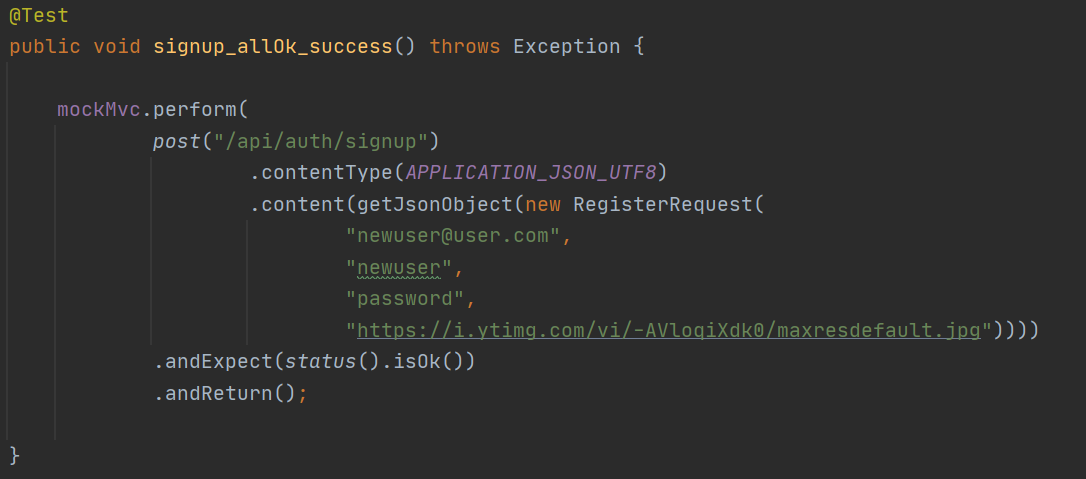
\includegraphics[scale=0.75]{slike/test1} \\
				\caption{ Test registracije u sustav ispravnim podacima}
				\label{fig:test1}
			\end{figure}
		
		
			\subsubsection{Test 2: Neuspješna registracija u sustav radi zauzetog korisničkog imena}
			Korisnik se pokuša registrirati u sustav imenom koje je zauzeto. \\
			Poslužitelj javlja da registracija nije uspjela,
			a klijentu se prikazuje tost koji se pojavljuje u gornjem desnom kutu ekrana.
			
			\begin{figure}[H]
				\centering
				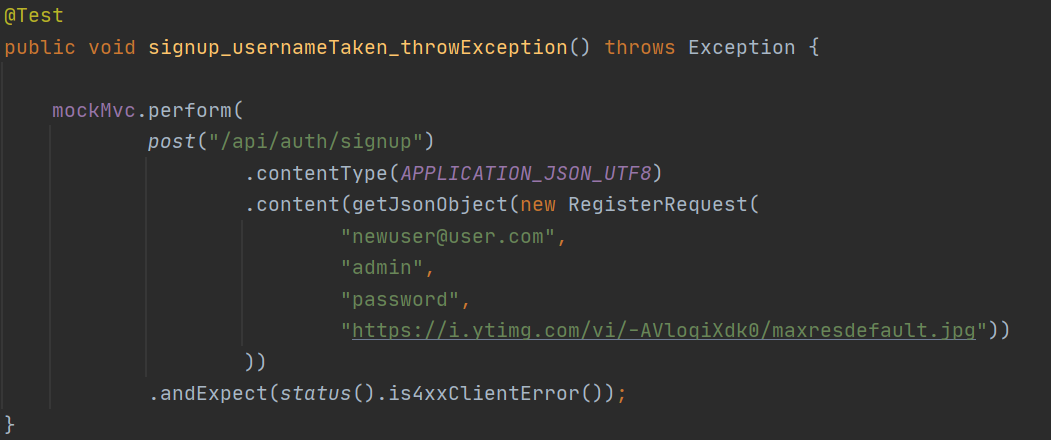
\includegraphics[scale=0.75]{slike/test2} \\
				\caption{ Test registracije u sustav zauzetim korisničkim imenom}
				\label{fig:test2}
			\end{figure}
		
			\subsubsection{Test 3: Neuspješna registracija u sustav radi lošeg URL-a slike}
			Korisnik se pokuša registrirati u sustav URL-om svoje slike koji je možda ispravno napisan, ali slika s tim URL-om nije dohvatljiva. \\
			Poslužitelj javlja da registracija nije uspjela, a klijentu se prikazuje tost koji se pojavljuje u gornjem desnom kutu ekrana.
			
			\begin{figure}[H]
				\centering
				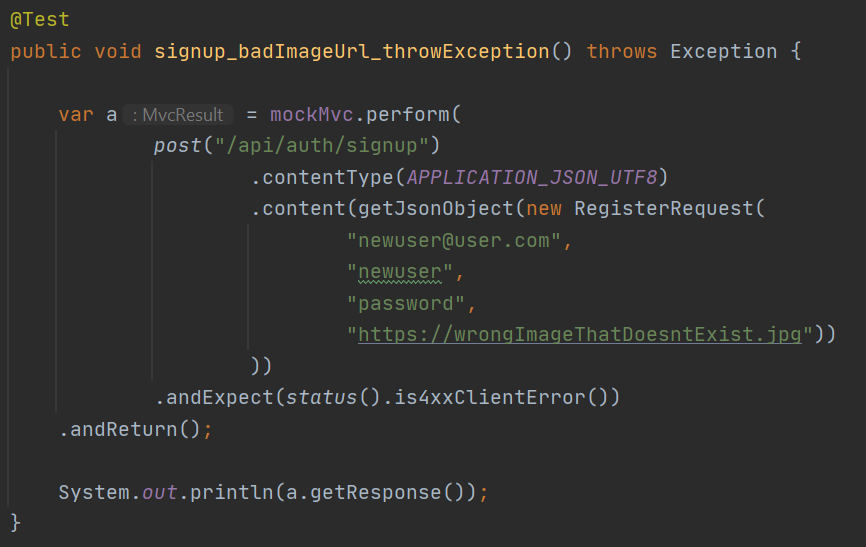
\includegraphics[scale=0.75]{slike/test3} \\
				\caption{ Test registracije u sustav lošim URL-om slike}
				\label{fig:test3}
			\end{figure}
		
			\subsubsection{Test 4: Uspješna prijava za kartografa}
			Korisnik se prijavljuje za kartografa u sustav IBAN brojem računa i URL-slikom svoje osobne iskaznice. \\
			U ovom testu su svi podatci ispravni, pa stoga poslužitelj treba uspješno pohraniti prijavu korisnika za kartografa i vratiti statusni kod 200 OK.
			
			\begin{figure}[H]
				\centering
				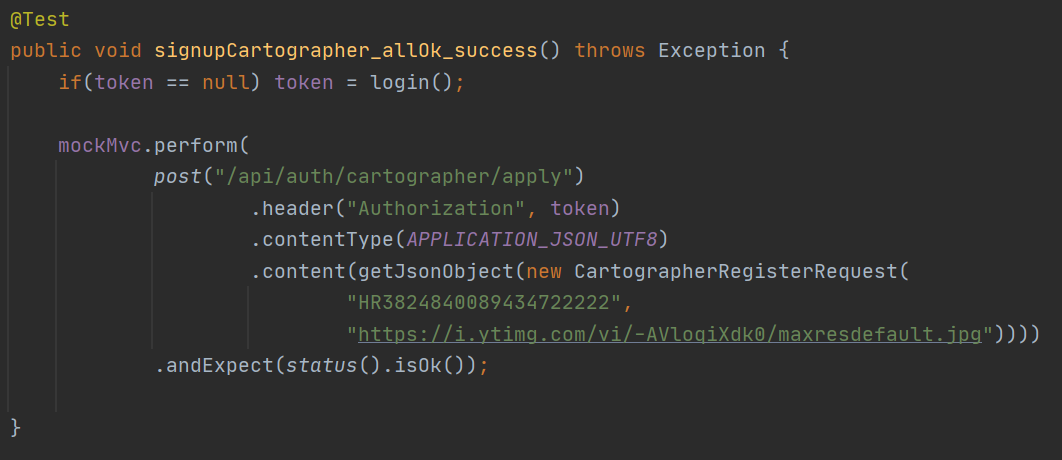
\includegraphics[scale=0.75]{slike/test4} \\
				\caption{ Test prijave za kartografa ispravnim podacima}
				\label{fig:test4}
			\end{figure}
		
			\subsubsection{Test 5: Uspješna prijava u sustav}
			Korisnik se prijavljuje u sustav korisničkim imenom i lozinkom. \\
			U ovom testu su svi podatci ispravni, pa stoga poslužitelj treba uspješno izvršiti prijavu korisnika i vratiti statusni kod 200 OK.
			
			\begin{figure}[H]
				\centering
				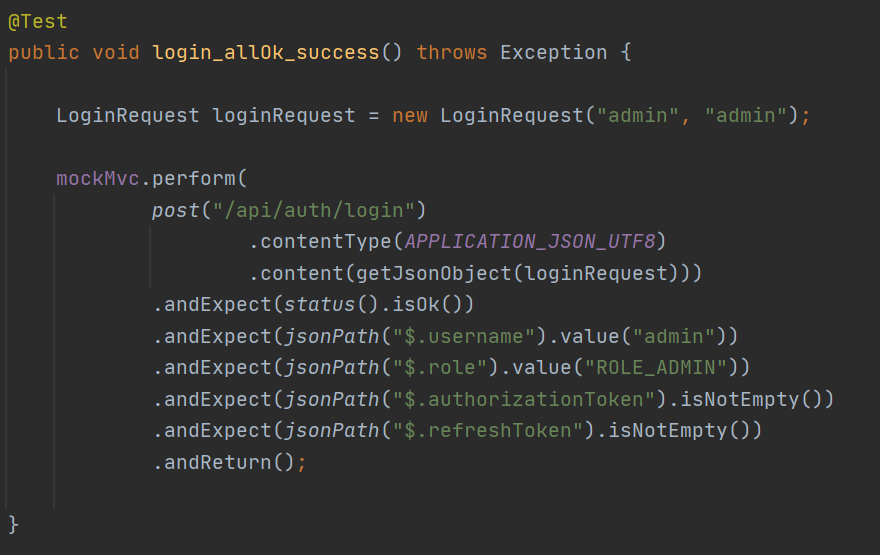
\includegraphics[scale=0.75]{slike/test5} \\
				\caption{ Test prijave u sustav ispravnim podacima}
				\label{fig:test5}
			\end{figure}
		
			\subsubsection{Test 6: Neuspješna prijava u sustav radi neispravnih podataka}
			Korisnik se pokuša prijaviti u sustav s neispravnom kombinacijom korisničkog imena i lozinke. \\
			Poslužitelj baca iznimku tipa BadCredentialsException a klijentu javlja da prijava nije uspjela.
			
			\begin{figure}[H]
				\centering
				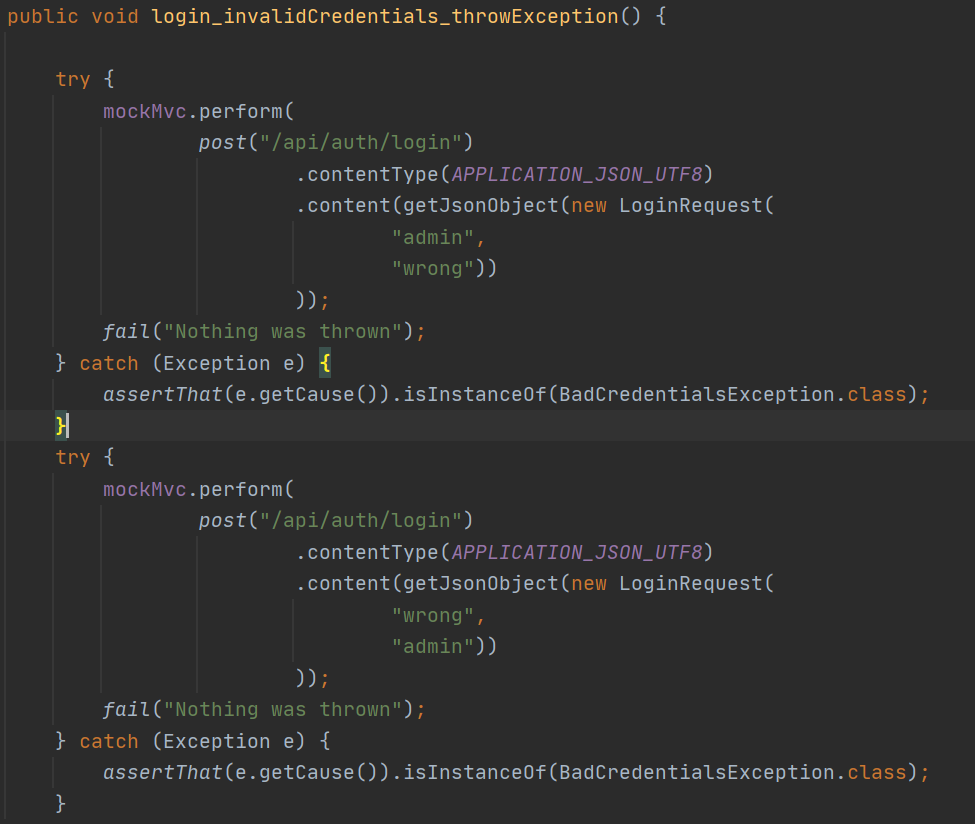
\includegraphics[scale=0.75]{slike/test6} \\
				\caption{ Test prijave u sustav neispravnim podacima}
				\label{fig:test6}
			\end{figure}
		
			\eject
		
			\subsubsection{Test 7: Parsiranje i ispisivanje koordinata}
			Ispitivanje metode koja parsira String u Point2D.Double u kojem čuvamo lokacije. \\
			Također ispitivanje da se lokacija iz klase Point2D.Double dobro ispisuje kao string.
		
			\begin{figure}[H]
				\centering
				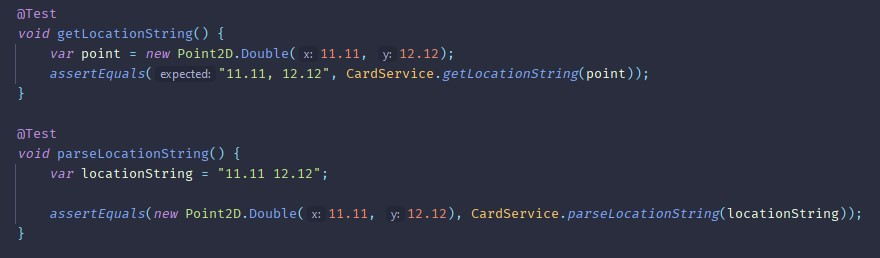
\includegraphics[scale=0.65]{slike/test7} \\
				\caption{ Test parsiranja i pretvaranja lokacije u String }
				\label{fig:test7}
			\end{figure}
		
			\subsubsection{Test 8: Osvajanje karte ne radi ako je igrač predaleko od nje}
			Ispitivanje metode koja se poziva prilikom osvajanja karte i očekivanje da će baciti exception koji znači da se karta nije mogla osvojiti zbog udaljenosti od igrača.
			
			\begin{figure}[H]
				\centering
				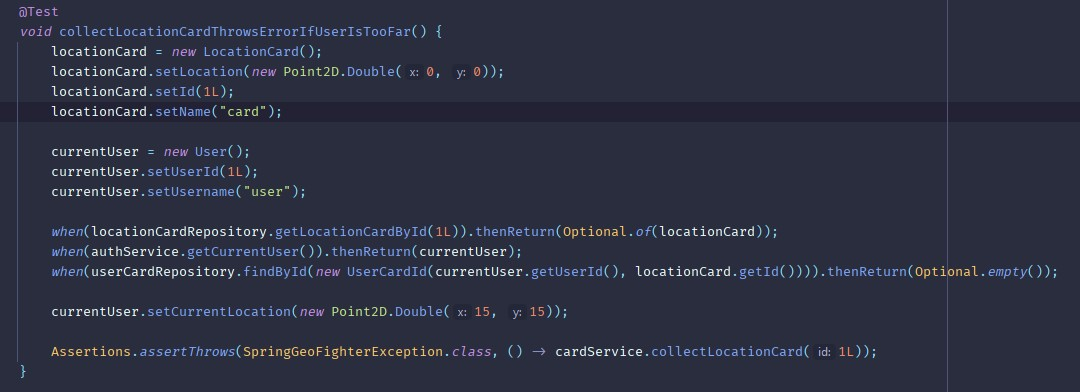
\includegraphics[scale=0.55]{slike/test8} \\
				\caption{ Test osvajanja karte koji baca exception ako je igrač predaleko }
				\label{fig:test8}
			\end{figure}
		
			\subsubsection{Test 9: Osvajanje karte ne radi ništa ako je igrač već ima}
			Ispitivanje metode koja se poziva prilikom osvajanja karte i očekivanje da ona neće napraviti nikakvu akciju spremanja u bazu podataka ukoliko igrač već posjeduje navedenu kartu.
			
			\begin{figure}[H]
				\centering
				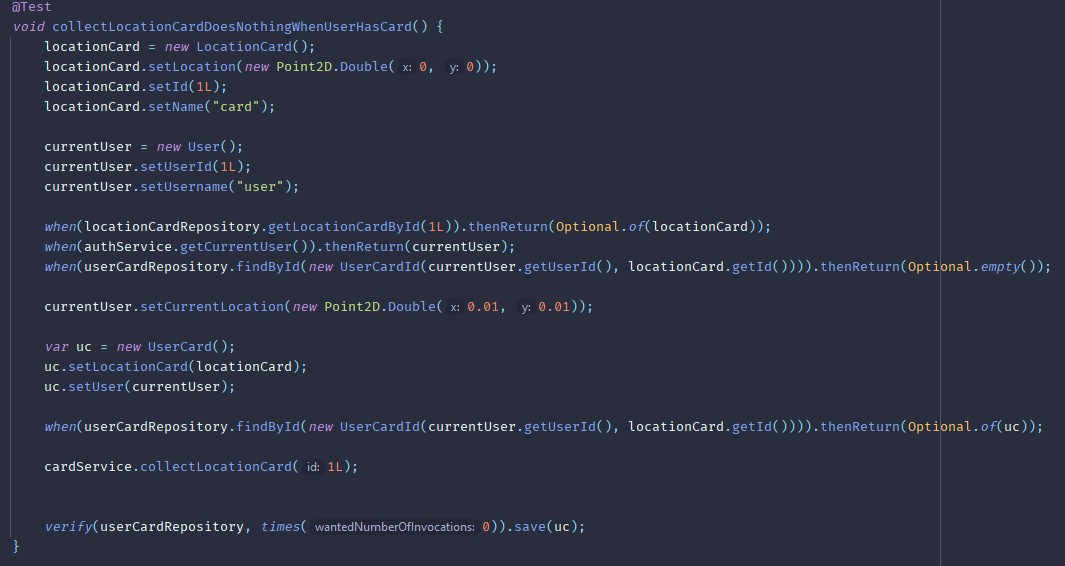
\includegraphics[scale=0.55]{slike/test9} \\
				\caption{ Test osvajanja karte koji provjerava da se ne poziva spremanje u bazu ako igrač posjeduje kartu}
				\label{fig:test9}
			\end{figure}
		
			\subsubsection{Test 10: Osvajanje karte uspješno sprema kartu}
			Ispitivanje metode uspješnog spremanja relacije karta-igrač u bazu podataka kod njenog osvajanja.
			
			\begin{figure}[H]
				\centering
				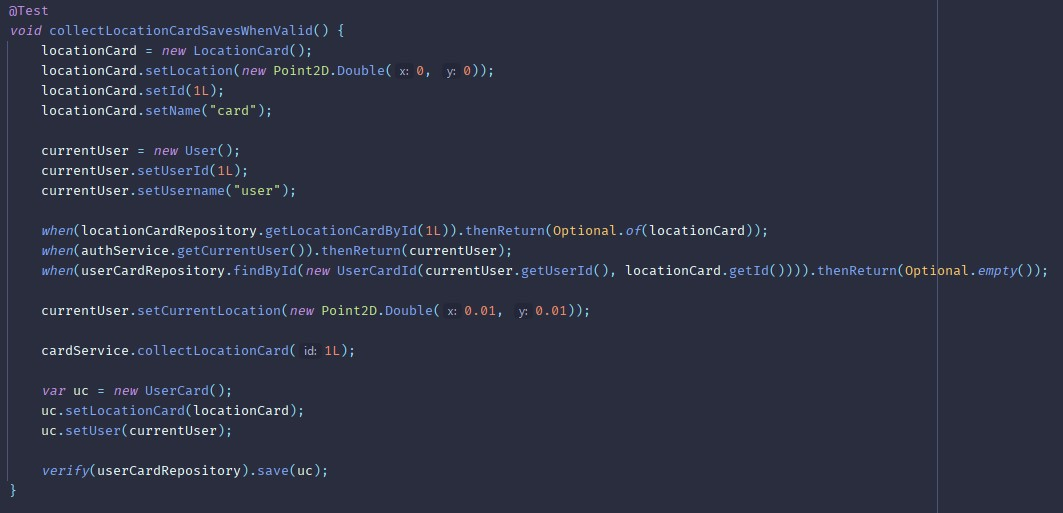
\includegraphics[scale=0.55]{slike/test10} \\
				\caption{ Test uspješnog spremanja u bazu podataka kod osvajanja}
				\label{fig:test10}
			\end{figure}
		
			\subsubsection{Test 11: Test računanja daljine između dvije lokacije}
			Ispitivanje metode koja računa zračnu udaljenost između dvije geografske lokacije.
			Lokacija se uspoređuje s poznatom udaljenosti u kilometrima između neke dvije točke.
			
			\begin{figure}[H]
				\centering
				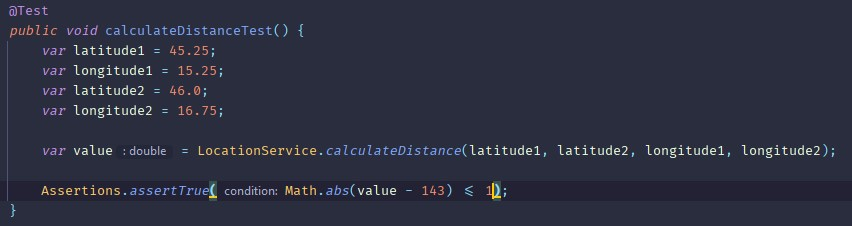
\includegraphics[scale=0.70]{slike/test11} \\
				\caption{ Test uspješnog spremanja u bazu podataka kod osvajanja}
				\label{fig:test10}
			\end{figure}
			
			\begin{figure}[H]
				\centering
				
\includegraphics[scale=1]{slike/ishodTestova} \\
				\caption{ Rezultati izvođenja svih napisanih testova}
				\label{fig:ishodTestova}
			\end{figure}
			
			\eject
			
			\subsection{Ispitivanje sustava}
			
		    Za potrebe ispitivanja sustava, koristili smo Selenium IDE.
			\subsubsection{Test 1: Registracija korisnika}
			\textbf{Očekivano: } Klikom na gumb \textit{Sign Up} učitava se stranica s formom za unos podataka potrebnih za registraciju korisnika: \textit{e-mail adresa, korisničko ime, lozinka} te \textit{poveznica na sliku profila}.\\
			\textbf{Rezultat: } Korisnik  je  uspješno  registriran  u  bazu  podataka  ili  je  sustav  dojavio grešku.\\
			
			    Na slici 5.13. prikazana je poruka prilikom neuspješne registracije korisnika u sustav. Na slici 5.14. prikazan je uspješan test registracije u alatu Selenium.

			\begin{figure}[H]
				\centering
				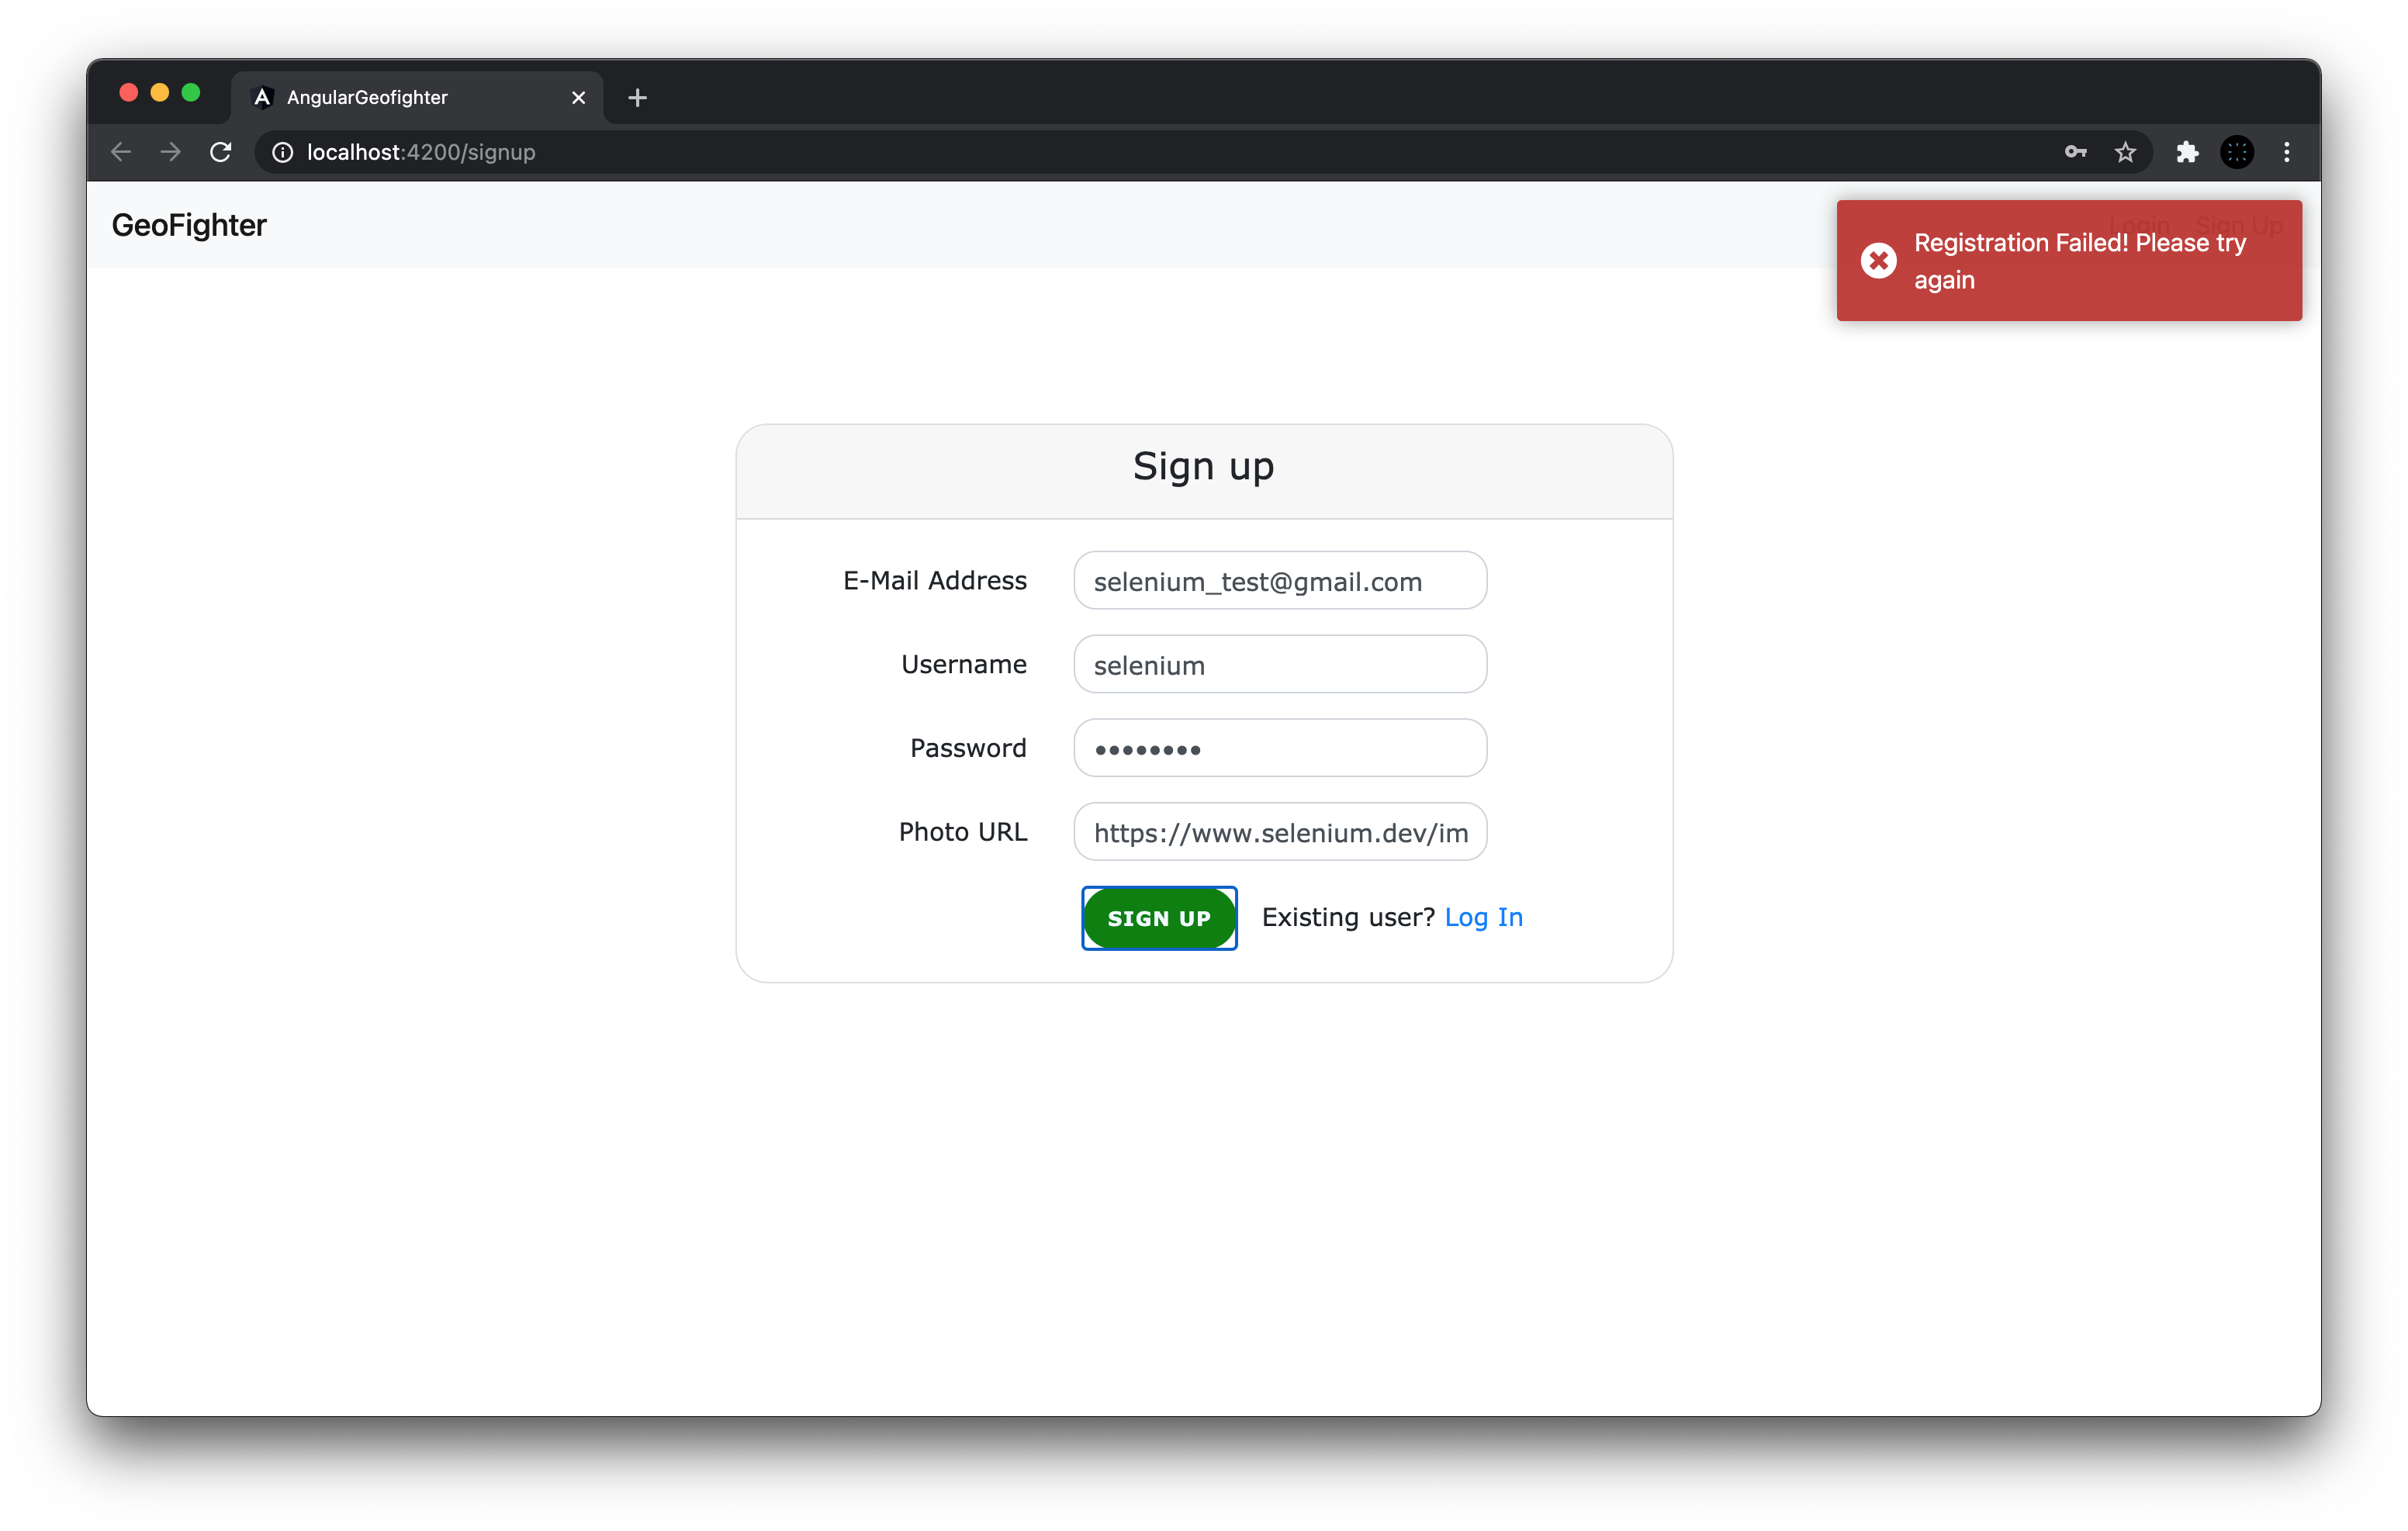
\includegraphics[scale=0.27]{slike/SeleniumRegistrationFail.png} \\
				\caption{ Prikaz poruke za neispravnu registraciju}
				\label{fig:SeleniumRegistrationFail}
			\end{figure}

			\begin{figure}[H]
				\centering
				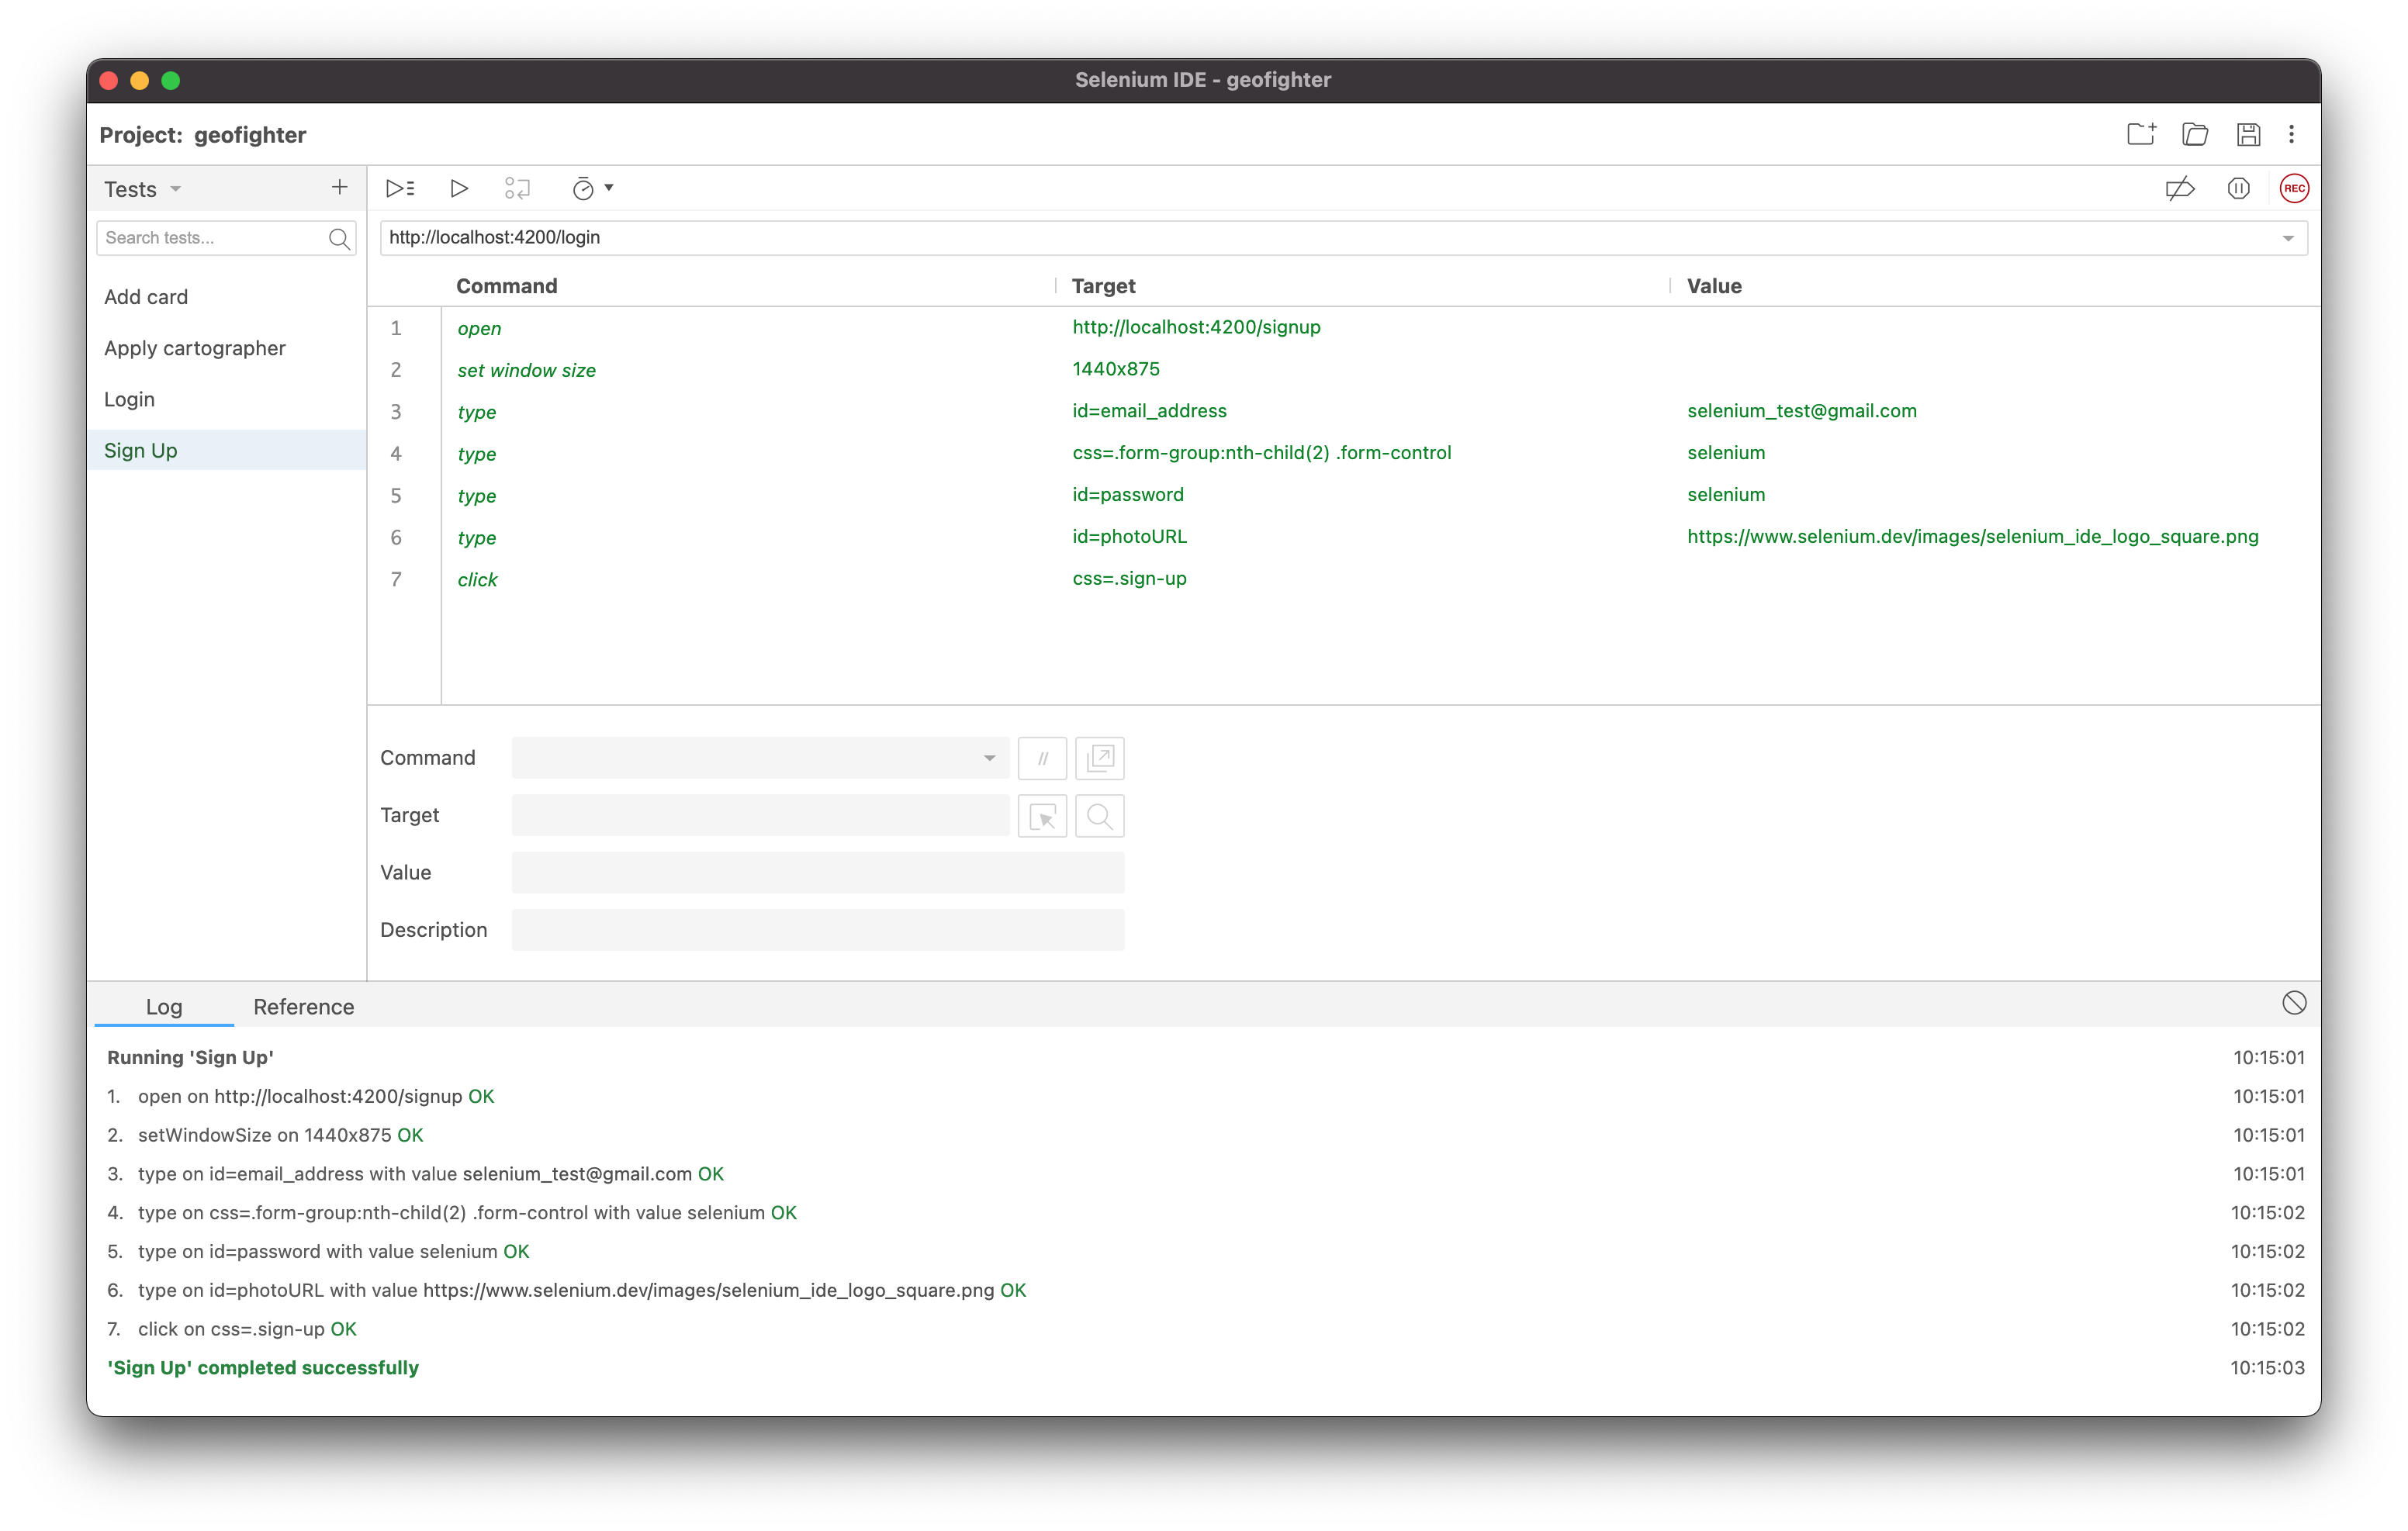
\includegraphics[scale=0.27]{slike/SeleniumRegistrationTest.png} \\
				\caption{ Selenium test koji prikazuje ispravnu registraciju}
				\label{fig:SeleniumRegistrationTest}
			\end{figure}

			\subsubsection{Test 2: Prijava korisnika u aplikaciju}
			\textbf{Očekivano: } Klikom na gumb \textit{Login} učitava se stranica s formom za unos podataka potrebnih za prijavu korisnika u aplikaciju: \textit{korisničko ime} i \textit{lozinka}.\\
			\textbf{Rezultat: } Korisnik  je  uspješno  prijavljen u aplikaciju ili  je  sustav  dojavio grešku.\\

			    Na slici 5.15. prikazan je prozor unutar aplikacije nakon uspješne prijave u aplikaciju. Na slici 5.16. prikazan je uspješan test prijave u aplikaciju u alatu Selenium.

			\begin{figure}[H]
				\centering
				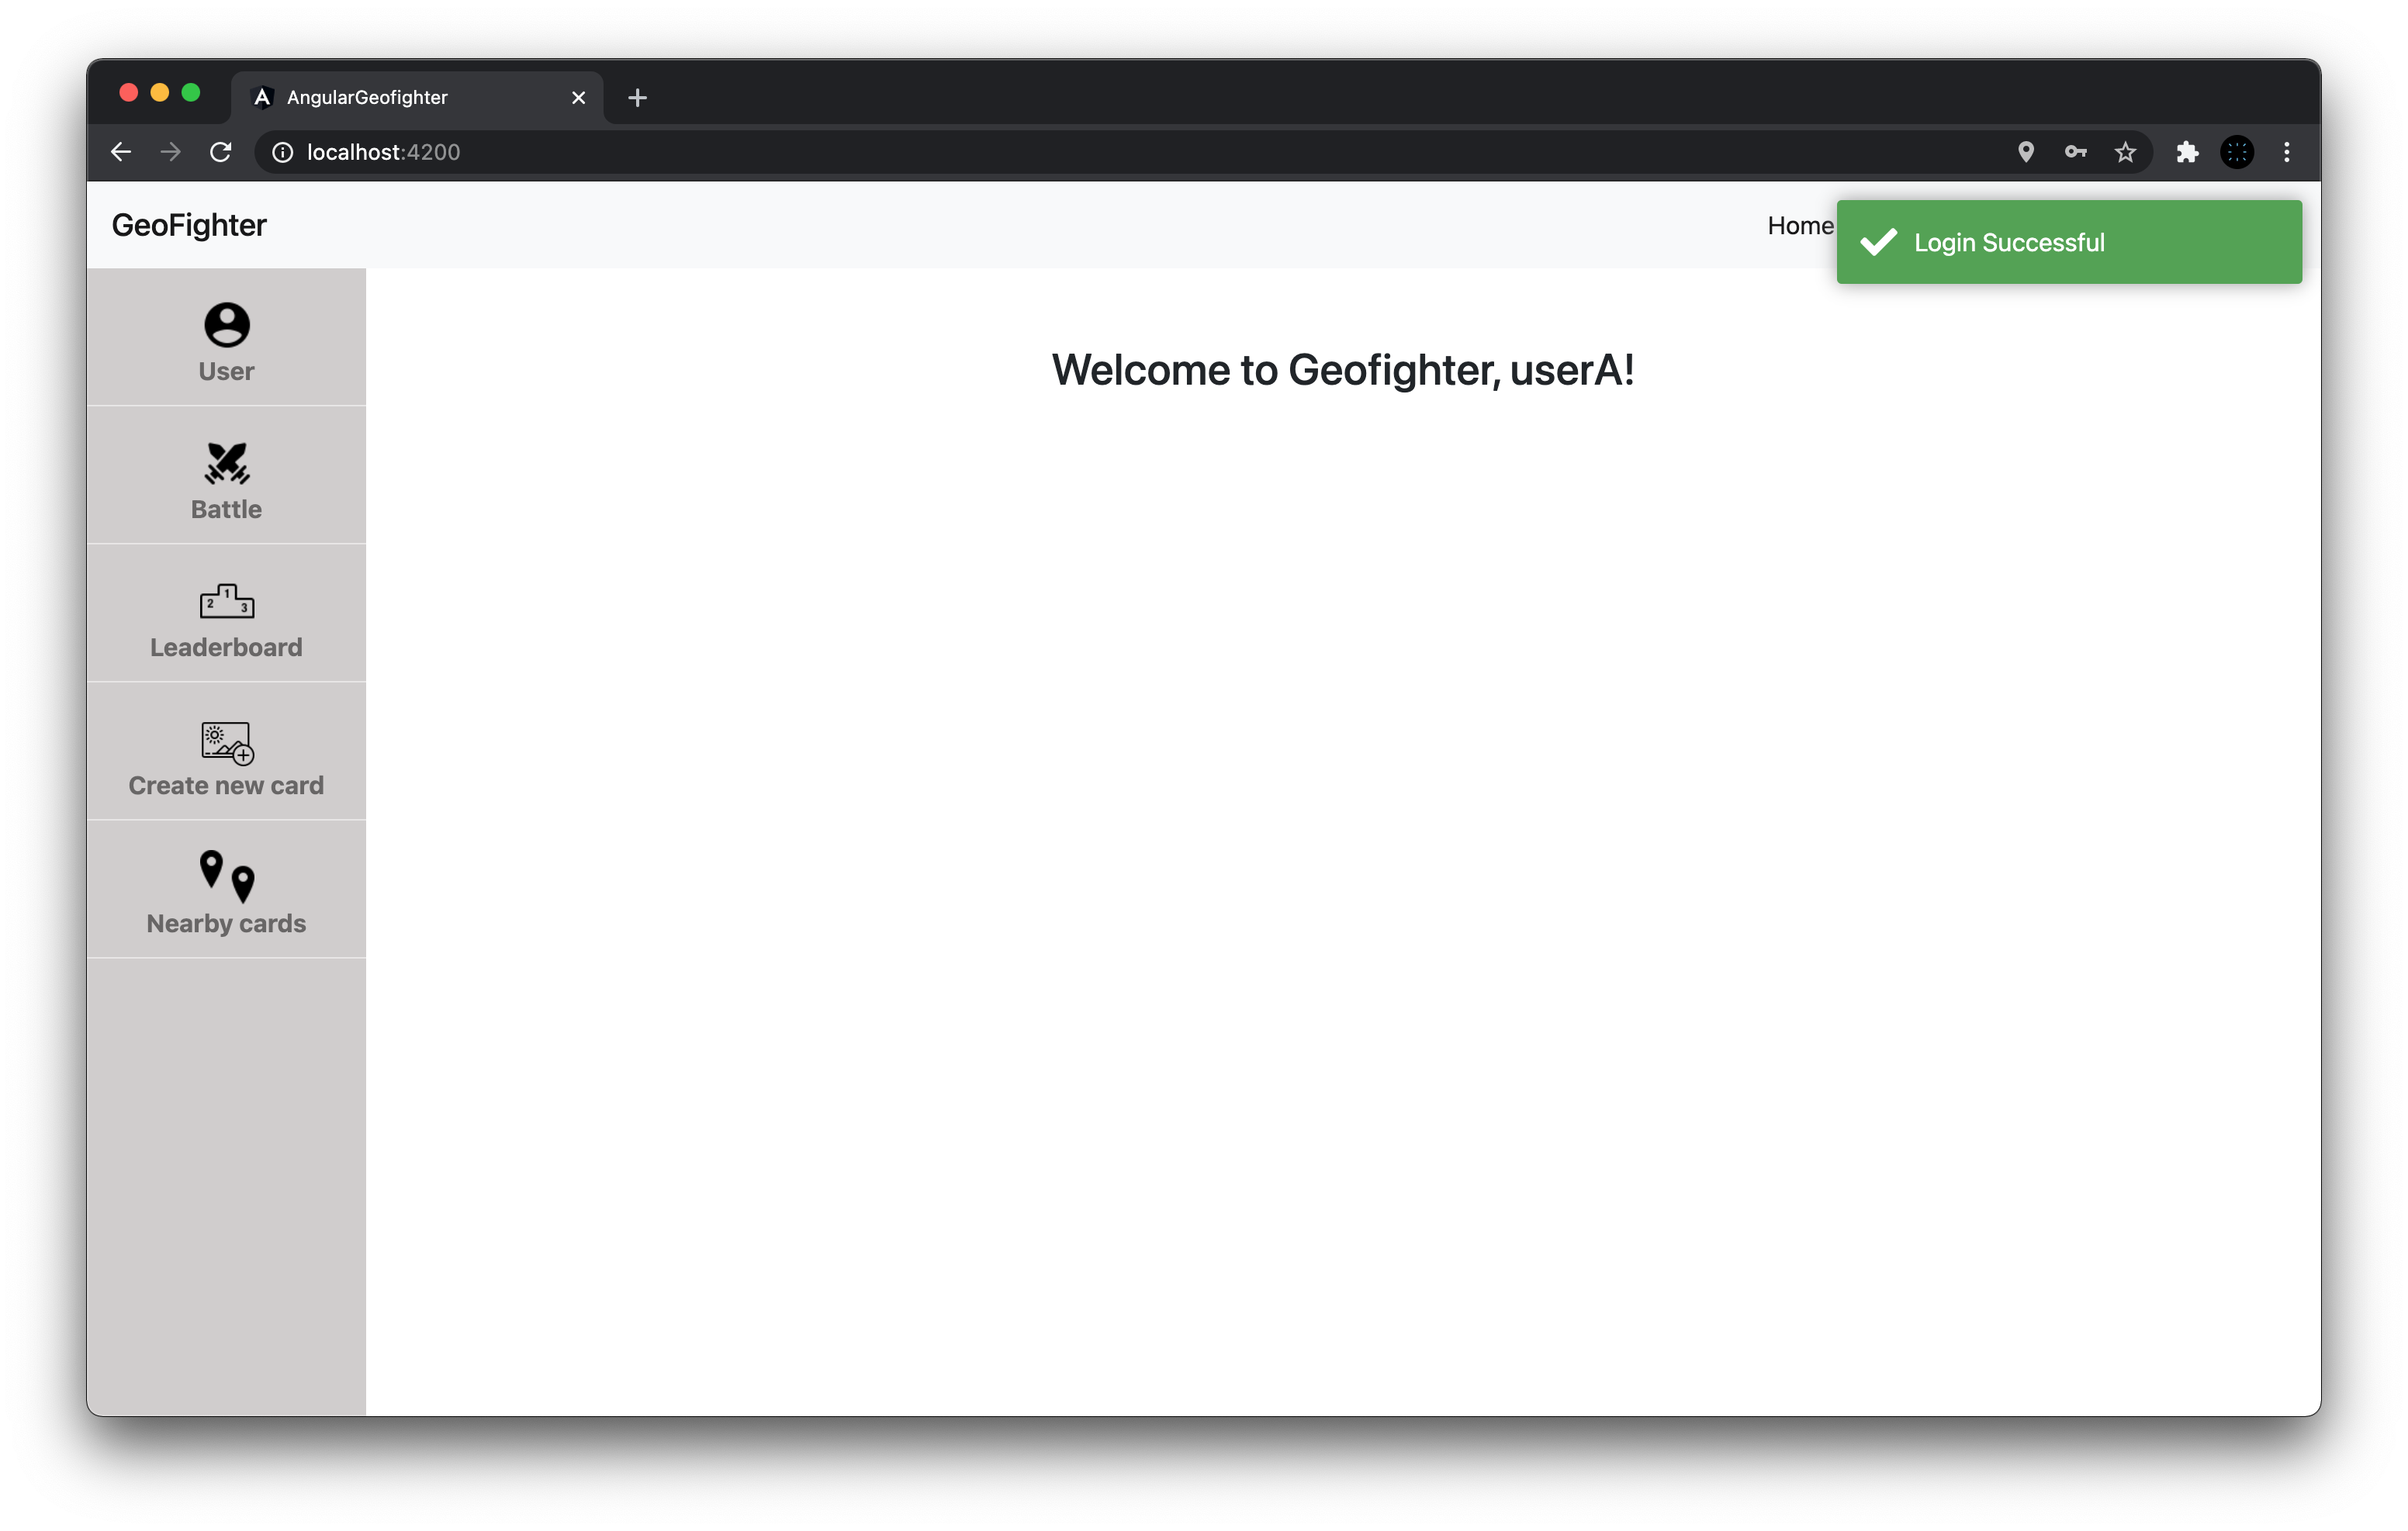
\includegraphics[scale=0.27]{slike/SeleniumLoginSuccess.png} \\
				\caption{ Prozor nakon uspješne prijave u aplikaciju}
				\label{fig:SeleniumLoginSuccess}
			\end{figure}

			\begin{figure}[H]
				\centering
				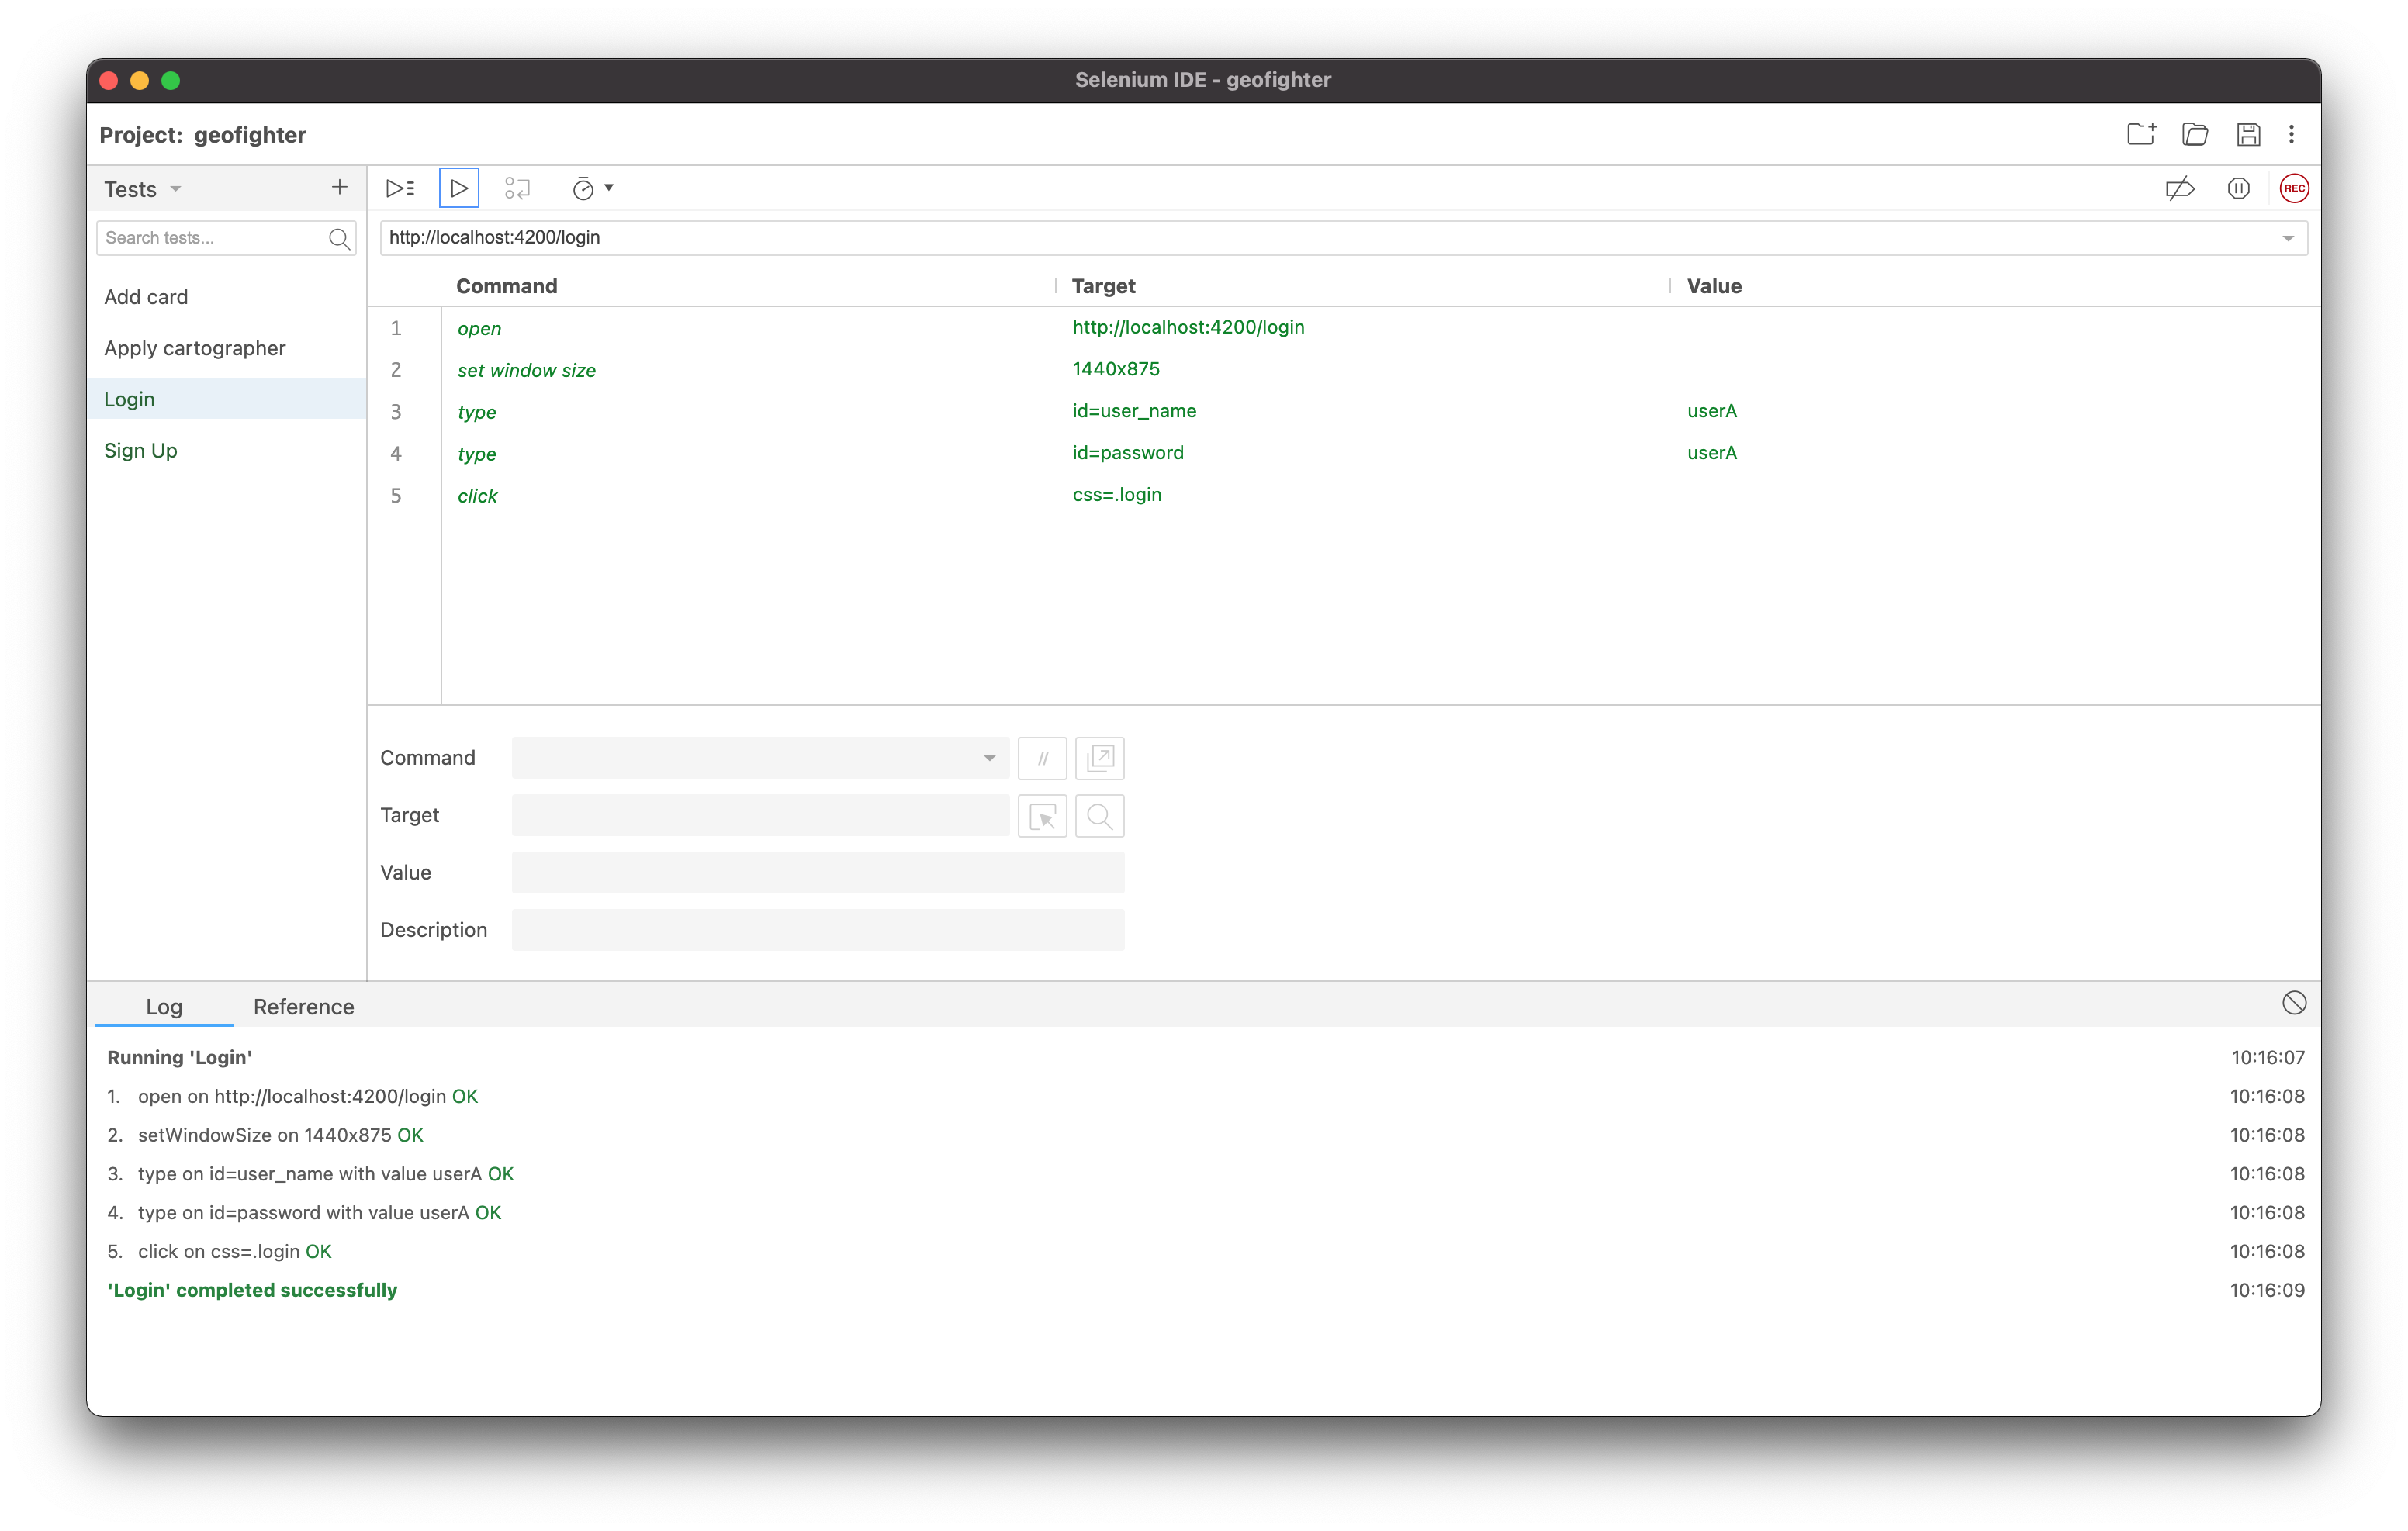
\includegraphics[scale=0.27]{slike/SeleniumLoginTest.png} \\
				\caption{ Selenium test koji prikazuje ispravnu prijavu u aplikaciju}
				\label{fig:SeleniumRegistrationFail}
			\end{figure}

			\subsubsection{Test 3: Prijava korisnika za poziciju kartografa}
			\textbf{Očekivano: } Nakon uspješne prijave korisnika u aplikaciju i nakon što korisnik stisne gumb \textit{Cartographer Apply} učitava se stranica s formom za unos podataka potrebnih za prijavu korisnika za poziciju kartografa: \textit{IBAN} i \textit{poveznica na sliku osobnog dokumenta}.\\
			\textbf{Rezultat: } Korisnik  se uspješno prijavio za poziciju kartografa ili  je  sustav  dojavio grešku.\\

			    Na slici 5.17. prikazana je poruka uspješne prijave za poziciju kartografa. Na slici 5.18. prikazan je uspješan test prijave za poziciju kartografa u alatu Selenium.

			\begin{figure}[H]
				\centering
				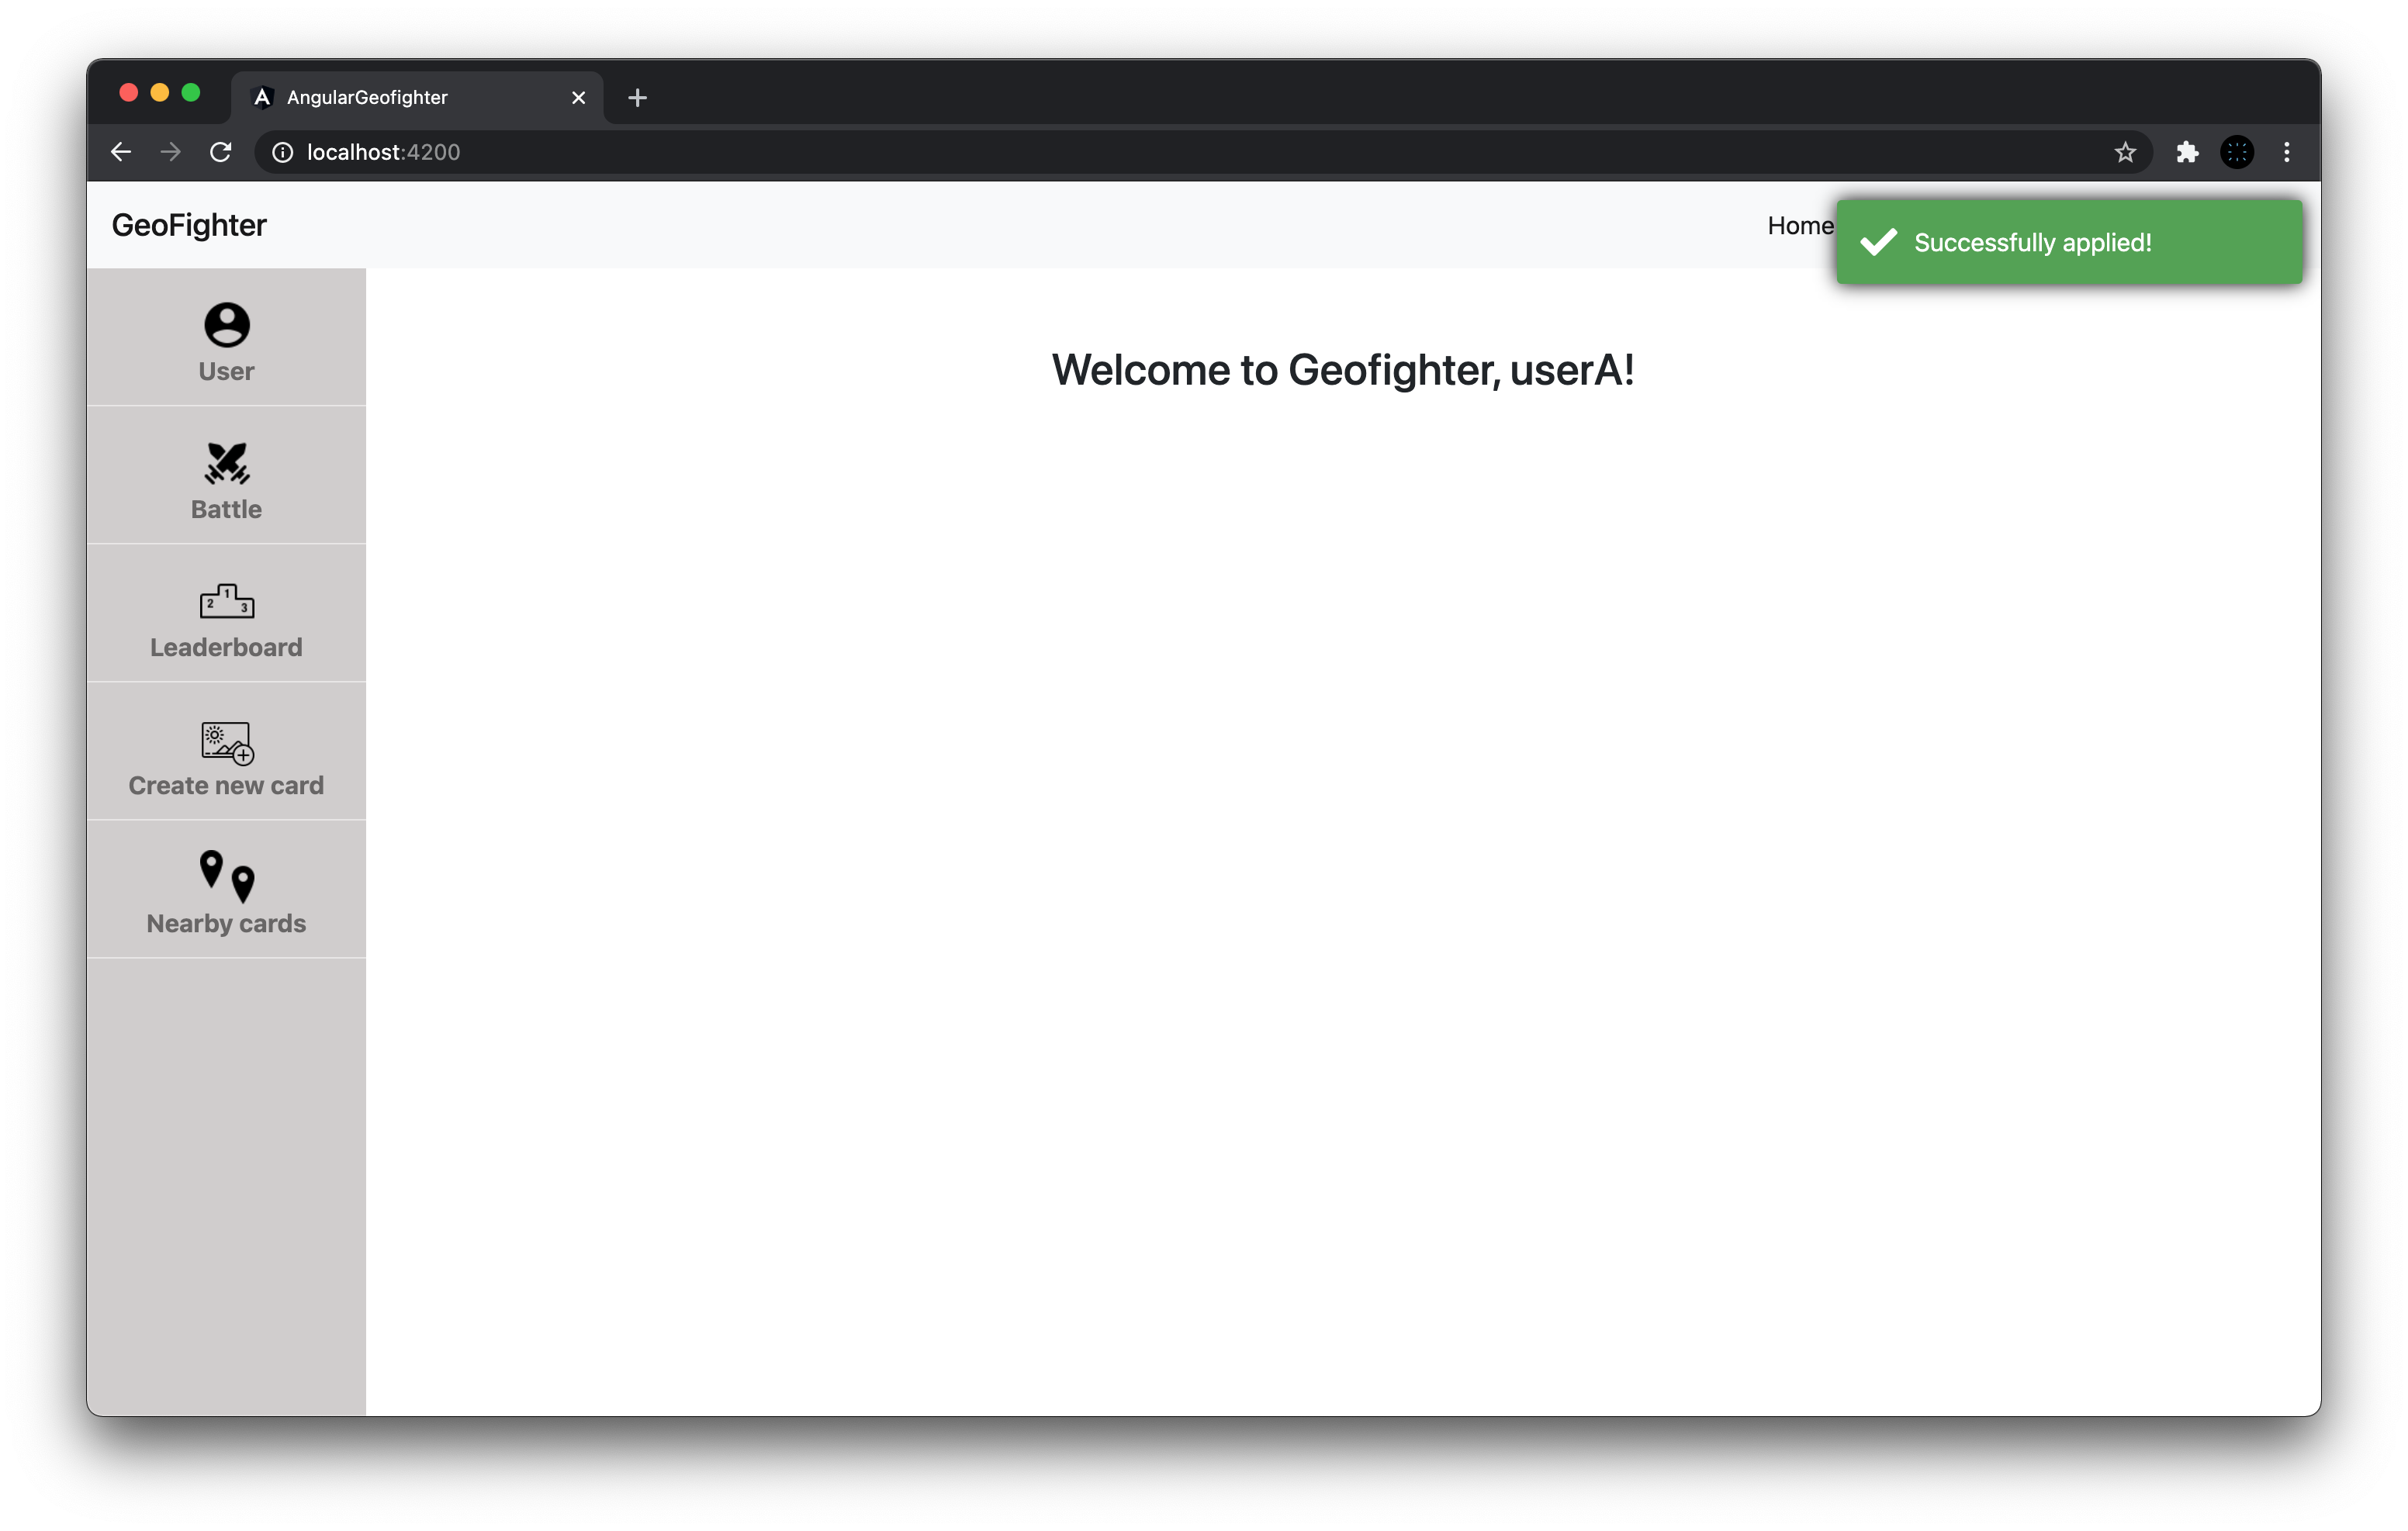
\includegraphics[scale=0.27]{slike/SeleniumCartographerSuccess.png} \\
				\caption{ Prozor nakon uspješne prijave korisnika za poziciju kartografa}
				\label{fig:SeleniumCartographerSuccess}
			\end{figure}

			\begin{figure}[H]
				\centering
				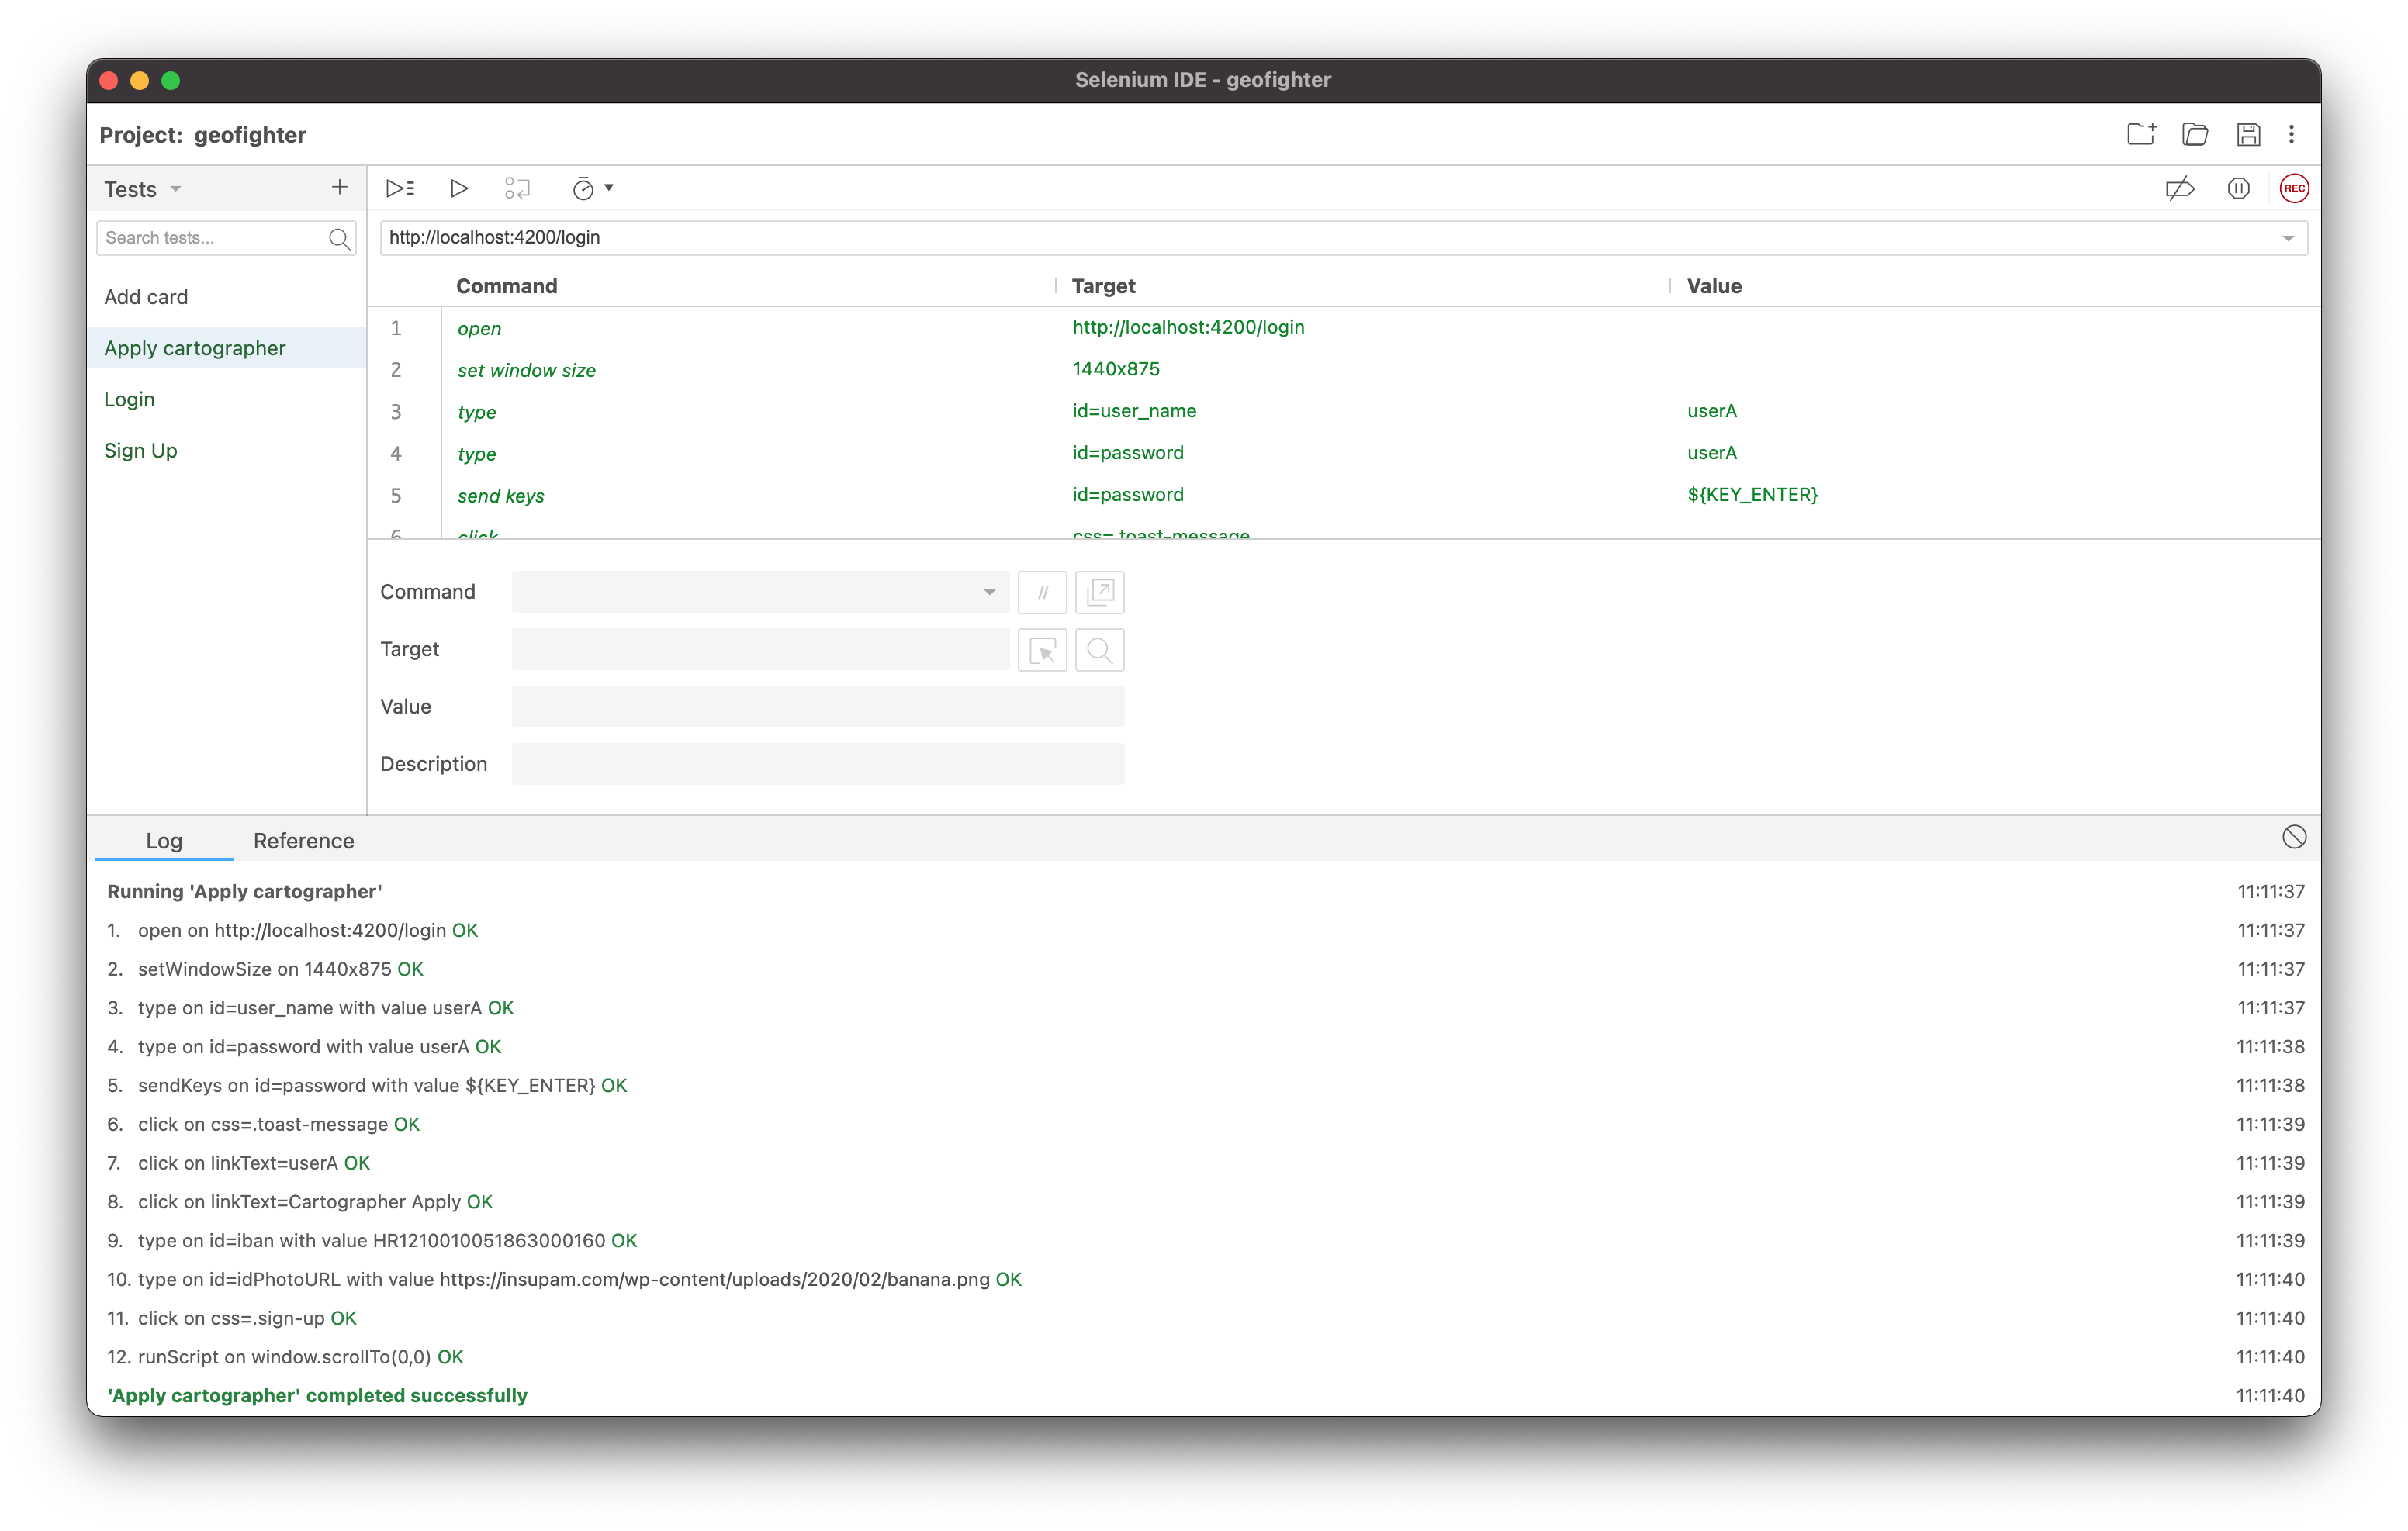
\includegraphics[scale=0.27]{slike/SeleniumCartographerTest.png} \\
				\caption{ Selenium test koji prikazuje ispravnu prijavu korisnika za poziciju kartografa}
				\label{fig:SeleniumCartographerTest}
			\end{figure}

			\subsubsection{Test 4: Dodavanje nove karte u sustav}
			\textbf{Očekivano: } Nakon uspješne prijave korisnika u aplikaciju i nakon što korisnik stisne gumb \textit{Create new card} učitava se stranica s formom za unos podataka potrebnih za dodavanje nove karte u sustav: \textit{naziv, opis, poveznica na sliku lokacije} i vrijednost za 3 parametra jačine karte:  \textit{dostupnost, popularnost, rijetkost}.\\
			\textbf{Rezultat: } Korisnik  je uspješno dodao prijavu za novu kartu ili  je  sustav  dojavio grešku.\\

			\begin{figure}[H]
				\centering
				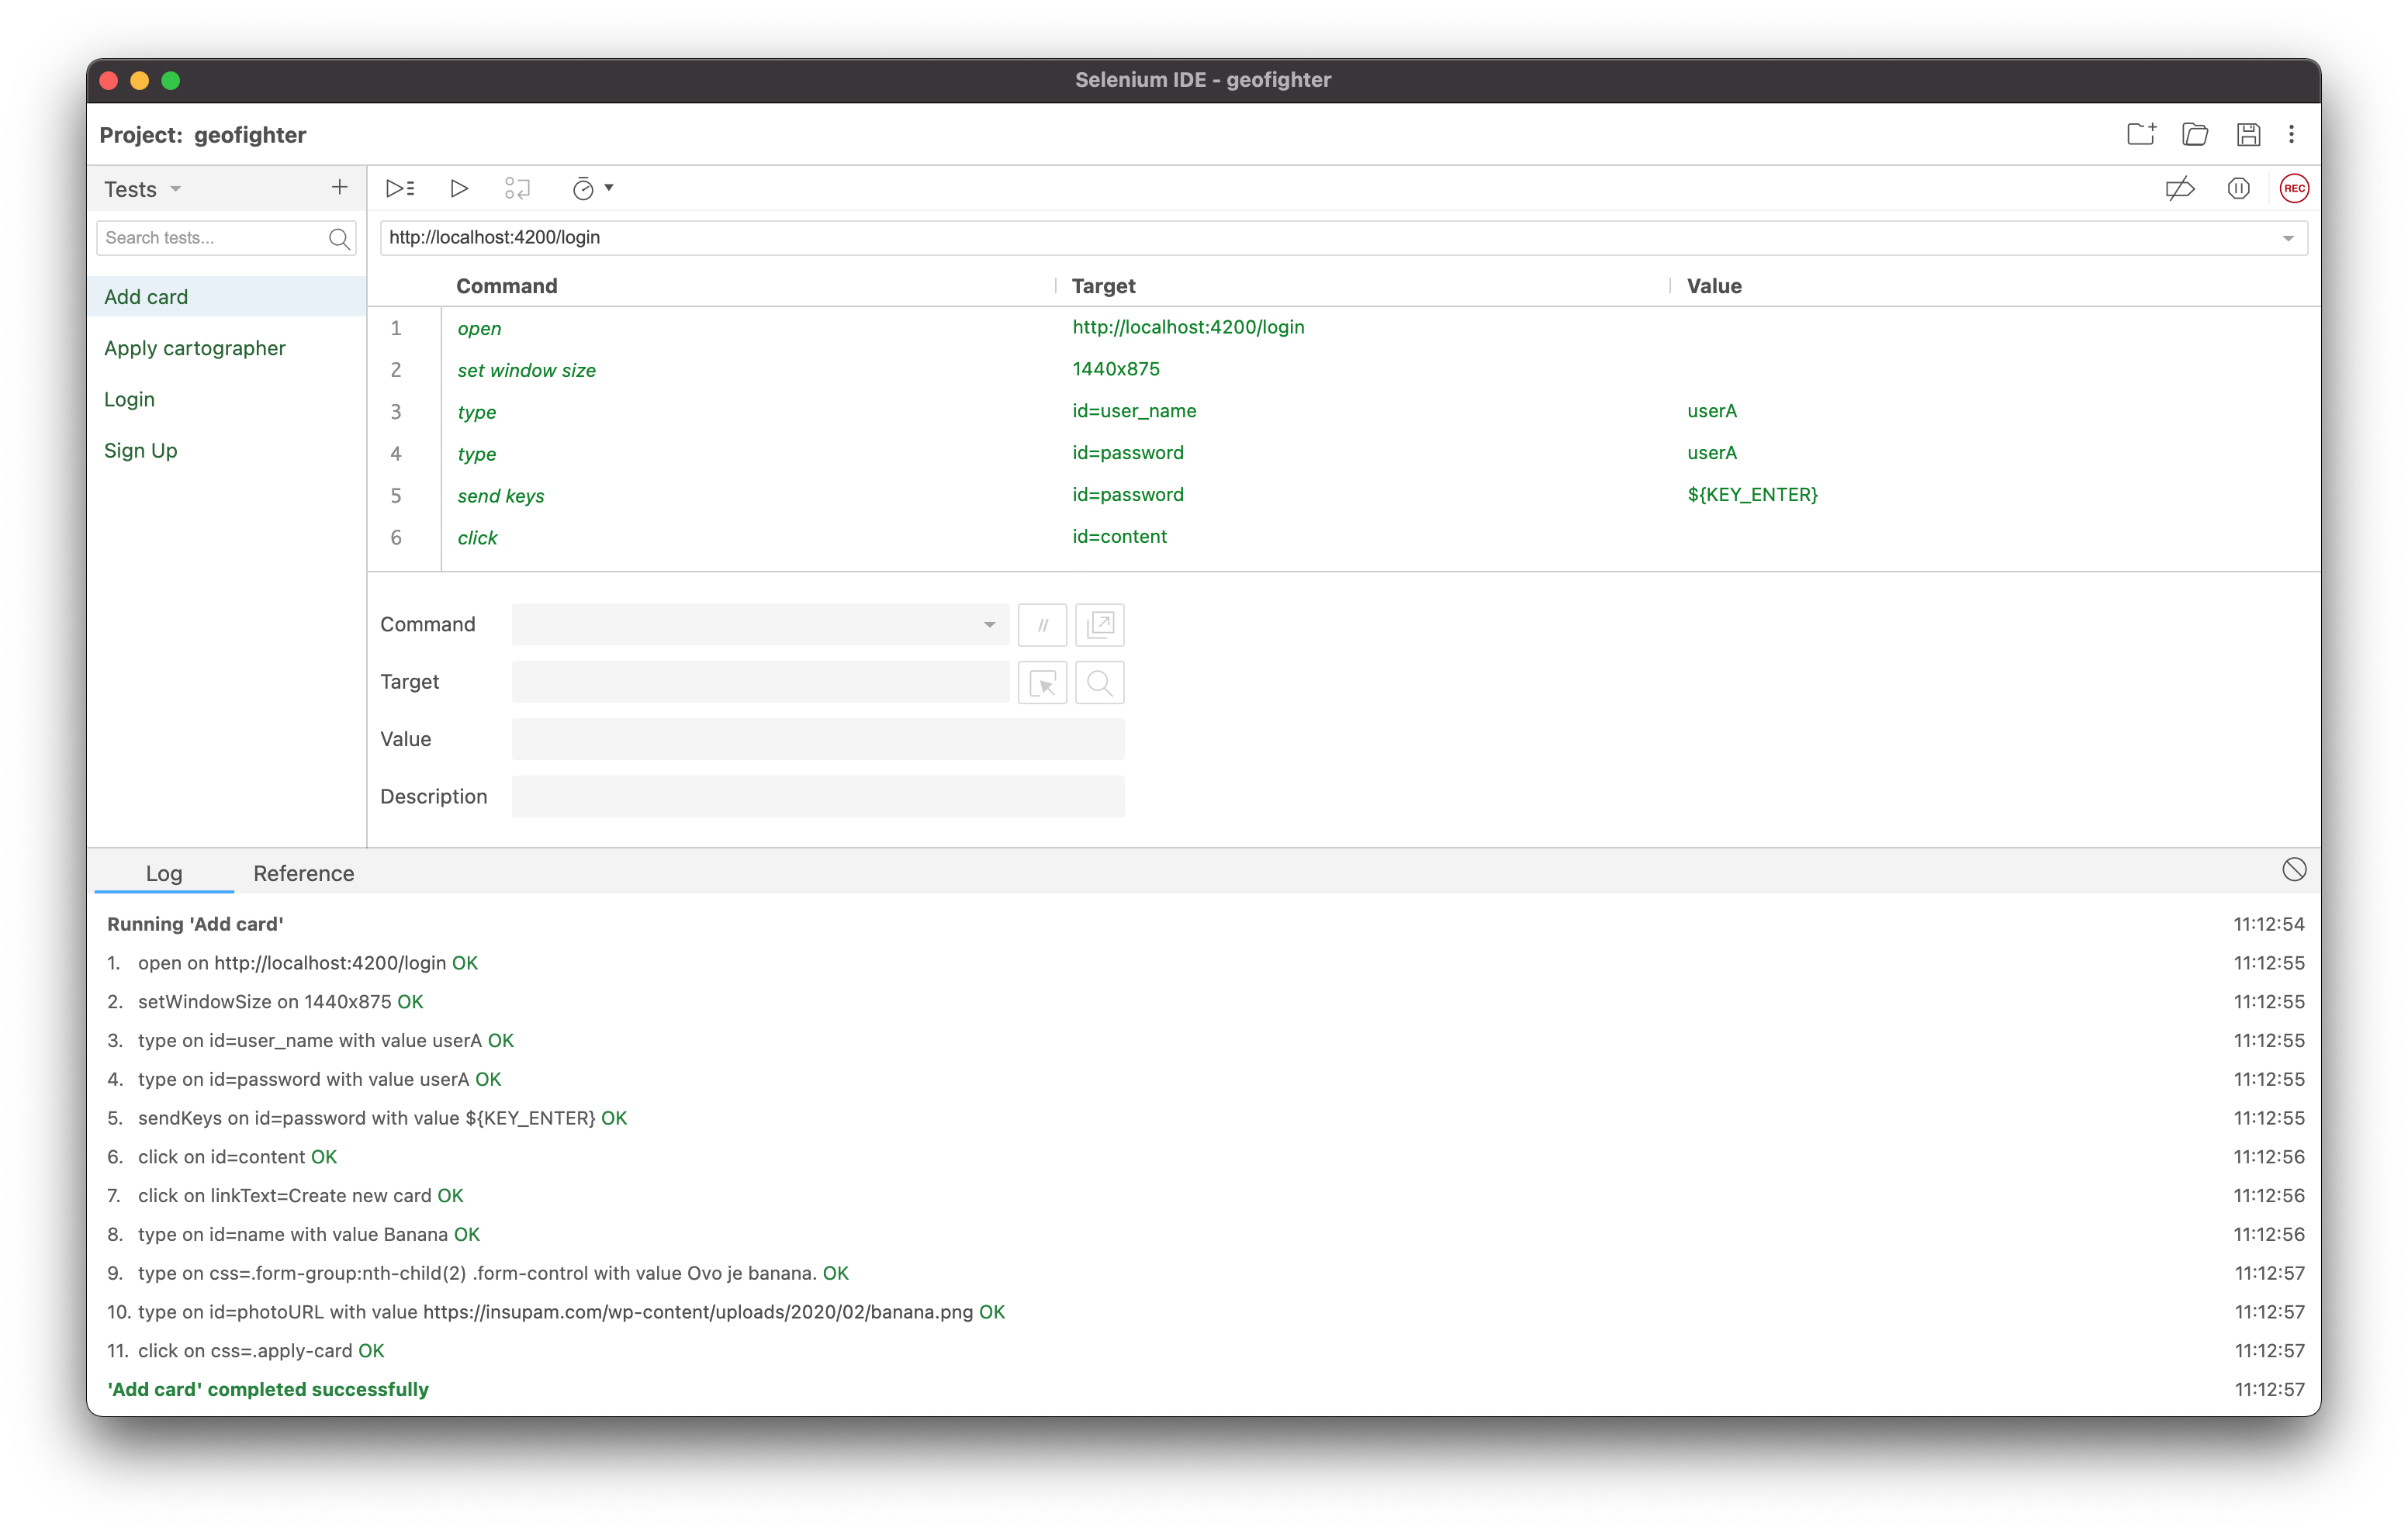
\includegraphics[scale=0.27]{slike/SeleniumCardSuccess.png} \\
				\caption{ Selenium test koji prikazuje ispravno dodavanje karte u sustav}
				\label{fig:SeleniumCartographerSuccess}
			\end{figure}

		    \eject
		
		
		\section{Dijagram razmještaja}
			
			 \textnormal{Dijagram razmještaja opisuje topologiju sklopovlja i programsku potporu koja se koristi u implementaciji sustava u njegovom radnom okruženju. Komponente programske potpore deployane su na oblak platformu Heroku. Heroku je platforma (PaaS) koja razvojnim programerima omogućuje izgradnju, pokretanje i upravljanje aplikacijama u potpunosti u oblaku. Sustav je baziran na arhitekturi klijent - poslužitelj. Komunikacija između njih odvija se HTTP protokolom.}
			
			
			\begin{figure}[H]
				\centering
				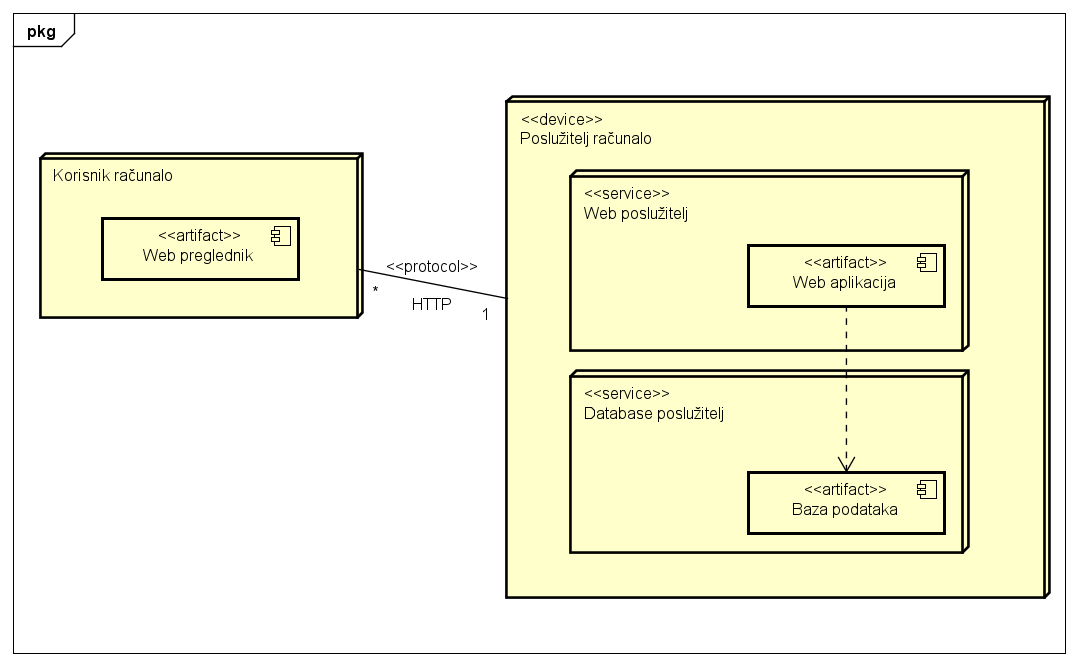
\includegraphics[scale=0.58]{dijagrami/Deployment Diagram0} \\
				\caption{Dijagram razmještaja}
				\label{fig:UC8_sekvencijski}
			\end{figure}
		
			\eject
		
		\section{Upute za puštanje u pogon}
		
			\textnormal{Za puštanje u pogon GeoFighter aplikacije iz izvornog kôda potrebno je nekoliko preduvjeta: \textbf{PostgreSQL13, JDK11 i Node.js 15}. Nakon što su navedene aplikacije preuzete i instalirane lako je kompilirati aplikaciju i pokrenuti ju na vlastitom računalu. Aplikacija je također pokrenuta na javno dostupnom poslužitelju \textbf{Heroku} o čemu piše više u nastavku.\\}
			
			\textbf{\textit{Koraci za pokretanje na lokalnom računalu:}}
			
			\begin{itemize}
				
				\item U PostgreSQL DBMS-u stvoriti novu bazu podataka te zapisati njeno ime (baze podataka) uz ime korisnika-vlasnika baze podataka, njegovu šifre i vrata (engl. port) baze.
				
				\item Unutar root direktorija otvoriti datoteku čiji je path\\ \textit{/izvorniKod/geoFighterSpring/src/main/resources/application-local.properties}\\ i unutar nje promijeniti sljedeće parametre: \begin{packed_enum}
					
					\item \textit{spring.datasource} parametre s parametrima novo-kreirane baze podataka. (Voditi brigu o portu, imenu baze podataka, te korisničkom imenu i lozinci vlasnika te baze)
					
					\item \textit{spring.mail} parametre s parametrima željenog mail servisa kako bi se mogli slati mailovi potvrde. Mail servis može biti javan kao što je trenutni \textit{gmail}, a moguće je koristiti testni kao što je \textit{mailtrap}\\ (\url{https://mailtrap.io})
				\end{packed_enum}
			
				\begin{figure}[H]
					\centering
					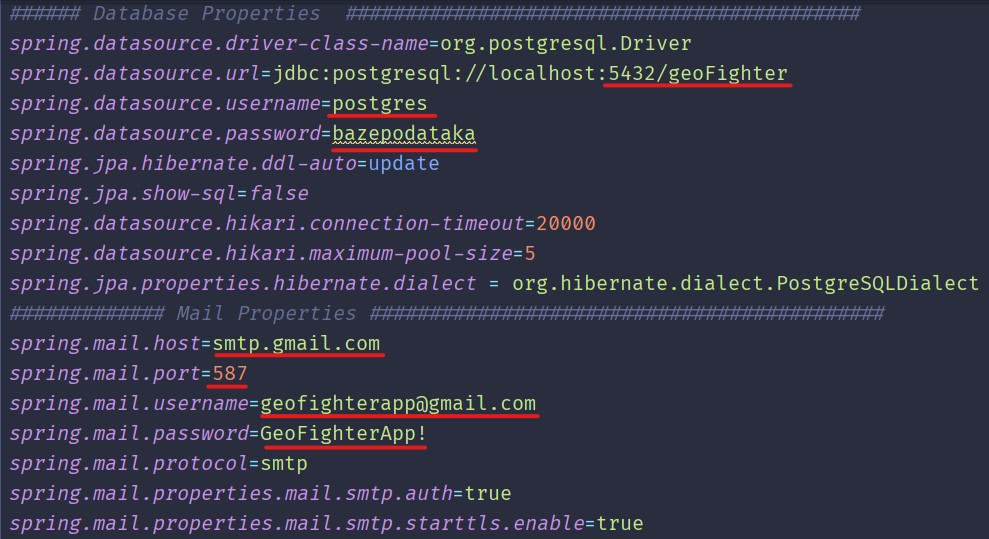
\includegraphics[scale=0.4]{slike/Properties} \\%veličina u odnosu na širinu linije
					\caption{Podatci koje je potrebno promijeniti u application-local.properties}
					\label{fig:properties} %label mora biti drugaciji za svaku sliku
				\end{figure}
			
				
				\item Otvoriti konzolu i pozicionirati se unutar \textit{/izvorniKod/geoFighterSpring/} i pokrenuti naredbu \textit{"./gradlew bootRun -Dspring.profiles.active=local"} s kojom se kompilira i zatim pokrene backend servis.
				
				\item Otvoriti drugu konzolu i pozicionirati se unutar \textit{/izvorniKod/angular-geofighter/} i pokrenuti naredbu \textit{"npm install"} kojom se preuzme i instalira sve potrebno za frontend servis. Zatim pokrenuti naredbu \textit{"ng build"}, te na kraju \textit{"npm start"} kojom se pokreće frontend servis na portu 4200.
				
				\item Ako su backend i frontend servis pokrenuti i u konzoli nisu dojavljene nikakve pogreške, aplikacija je spremna za korištenje na lokalnom računalu.\\\\
				
			\end{itemize}
		
			
			\textit{Aplikacija je puštena u pogon na javno dostupnom poslužitelju \textbf{Heroku} tako da su sve tri komponente (DB, FrontEnd i BackEnd) tamo pokrenute i moguće joj je pristupiti s linka:}\\
			\url{https://angularfrontend-release.herokuapp.com/}\\
						
			\textit{GitLab repozitorij \url{https://gitlab.com/MatejC_FER/pi} također sadrži implementiran CI/CD (Continuous integration and continuous delivery) pomoću kojeg se pri svakom commitu na \textbf{Master} branch automatski aplikacija izgradila i deployala na \textbf{Heroku} javni poslužitelj. Tako nije potrebno lokalno pokretati aplikaciju nakon izmjena, već je dovoljno na repozitorij pohraniti promjene.}
			
			
			\eject 